\chapter{Evaluation}\label{chap:evaluation}
In this chapter, we present our evaluation criteria and the findings which we got from them.
We evaluate the four models with a three-pronged strategy, targeting the following characteristics:

\begin{enumerate}
    \item\textbf{Accuracy} - the share of correct next-activity predictions
    \item\textbf{Training time} - the amount of time required for training
    \item\textbf{Stability} - the change in prediction accuracy with progress
\end{enumerate}

While the first two criteria target the general usability of each model, the last one permits making a judgment about the stability of the predictions. The works of Francescomarino et al.~\cite{francescomarino2015} and Klinkmüller et al.~\cite{klinkmuller2018reliablemonitoring}, inspired this measure. It provides an understanding of how the prediction accuracy of a model changes as the traces gets longer. This can facilitate building trust in the model, as indicated in the introduction of the thesis~\cite{klinkmuller2018reliablemonitoring, boehmer2018probability}.
During the evaluation, results for BPIC logs and the HelpDesk dataset should not be compared too closely, as the BPIC logs are a lot more resouceful in terms of data attributes.

We discuss the acurracy of the models in \autoref{sec:eval:accuracy}, followed by the discussion of the required training time in \autoref{sec:eval:training-time}. We go on to discuss stability in \autoref{sec:eval:stability}, and conclude the chapter in \autoref{sec:eval:discussion}.

\section{Accuracy}\label{sec:eval:accuracy}
The validation accuracy is a good indicator of the prediction performance of any prediction model. It is the share of correct predictions among the number of total predictions. We go over the model accuracies by batching strategy and explain the results. In \autoref{fig:max-accuracies-helpdesk} to \autoref{fig:max-accuracies-bpic2015-5}, the model performances per dataset are presented, grouped by batching strategy. The plots make apparent that only three models perform well consistently and that the batching strategies can have a profound effect on accuracy.\\

% individual batching strategy
The individual batching strategy often results in slightly worse accuracies than the grouped batching strategy. We trace this back to the more frequent adjustment of weights that can lead the loss optimization into local minima~\cite{keskar2016large}. For this strategy, the SCH model always gives the best accuracies. On HelpDesk, this strategy delivers among the best results, and on BPIC11 the worst. It seems that the strategy helps achieving better and better results with decreasing process complexity.

% grouped batching strategy
The grouped batching strategy generally leads to top performance in lieu with our SP2 model on any dataset except for BPIC11 and BPIC12. On BPIC11, the strategy brings the best accuracy with the PFS model. On BPIC12, it causes the worst accuracies on the dataset. The explanation for this can be found in \autoref{tab:dataset-characteristics} and \autoref{tab:batch-sizes}. The dataset has the highest number of traces, and a relatively even distribution of lengths, resulting in a small standard deviation. This results in too many traces being put in a single batch, causing lost optimization opportunities. With this in mind, the grouping strategy should be enhanced to split batches if they exceed a certain size threshold. Nonetheless, we realized that the mean of the top accuracies of the SCH, SP2 and PFS models is the highest with the grouping strategy. \autoref{tab:strategy-top-accuracies} illustrates these mean accuracies.
%We also realized that the grouping strategy not only contributes to the best accuracies but also that it has a harmonizing effect on the accuracies among the SCH, SP2 and PFS models. This effect is illustrated in \autoref{fig:accuracy-harmonization}. The heatmap shows how the standard deviation between the top accuracies of the three models decreases with the grouping strategy on any dataset.

% padded strategy
The padded strategy leads to consistently good results throughout the datasets and only loses accuracy only on the BPIC11 datasets where the training was shrunk because traces exceeded a length threshold.

% windowed strategy
The batching strategies that provide the whole history in one sample consistently see the SCH, SP2 and PFS models on par with at most $0.1$ difference. The windowed batching strategy leads to very different results, depending on the dataset and model. With a window size of three, as suggested by Schönig et al., the model does not have many timesteps to learn from in any given sample. However, this loss of information does not impact the SP2 model. We assume that its SP-2 features encode the history that is cut away and thus help it come close to the general maximum accuracy of any dataset - except on BPIC11.

Looking at the accuracy of the EVM model across all datasets, it is evident that it is consistently outperformed. We trace the low accuracy back to the application of an Embedding layer, which we suspect to require more data than included in most datasets to improve its internal data representation.
Its accuracy on the BPIC12 dataset represents an exception. The performance jump here corresponds to the small number of activities and a large number of traces in \autoref{tab:dataset-characteristics}, which could help the Embedding learn better. Therefore, we assume that Embeddings need more training data than currently available to become more effective.

\begin{figure}
    \centering
    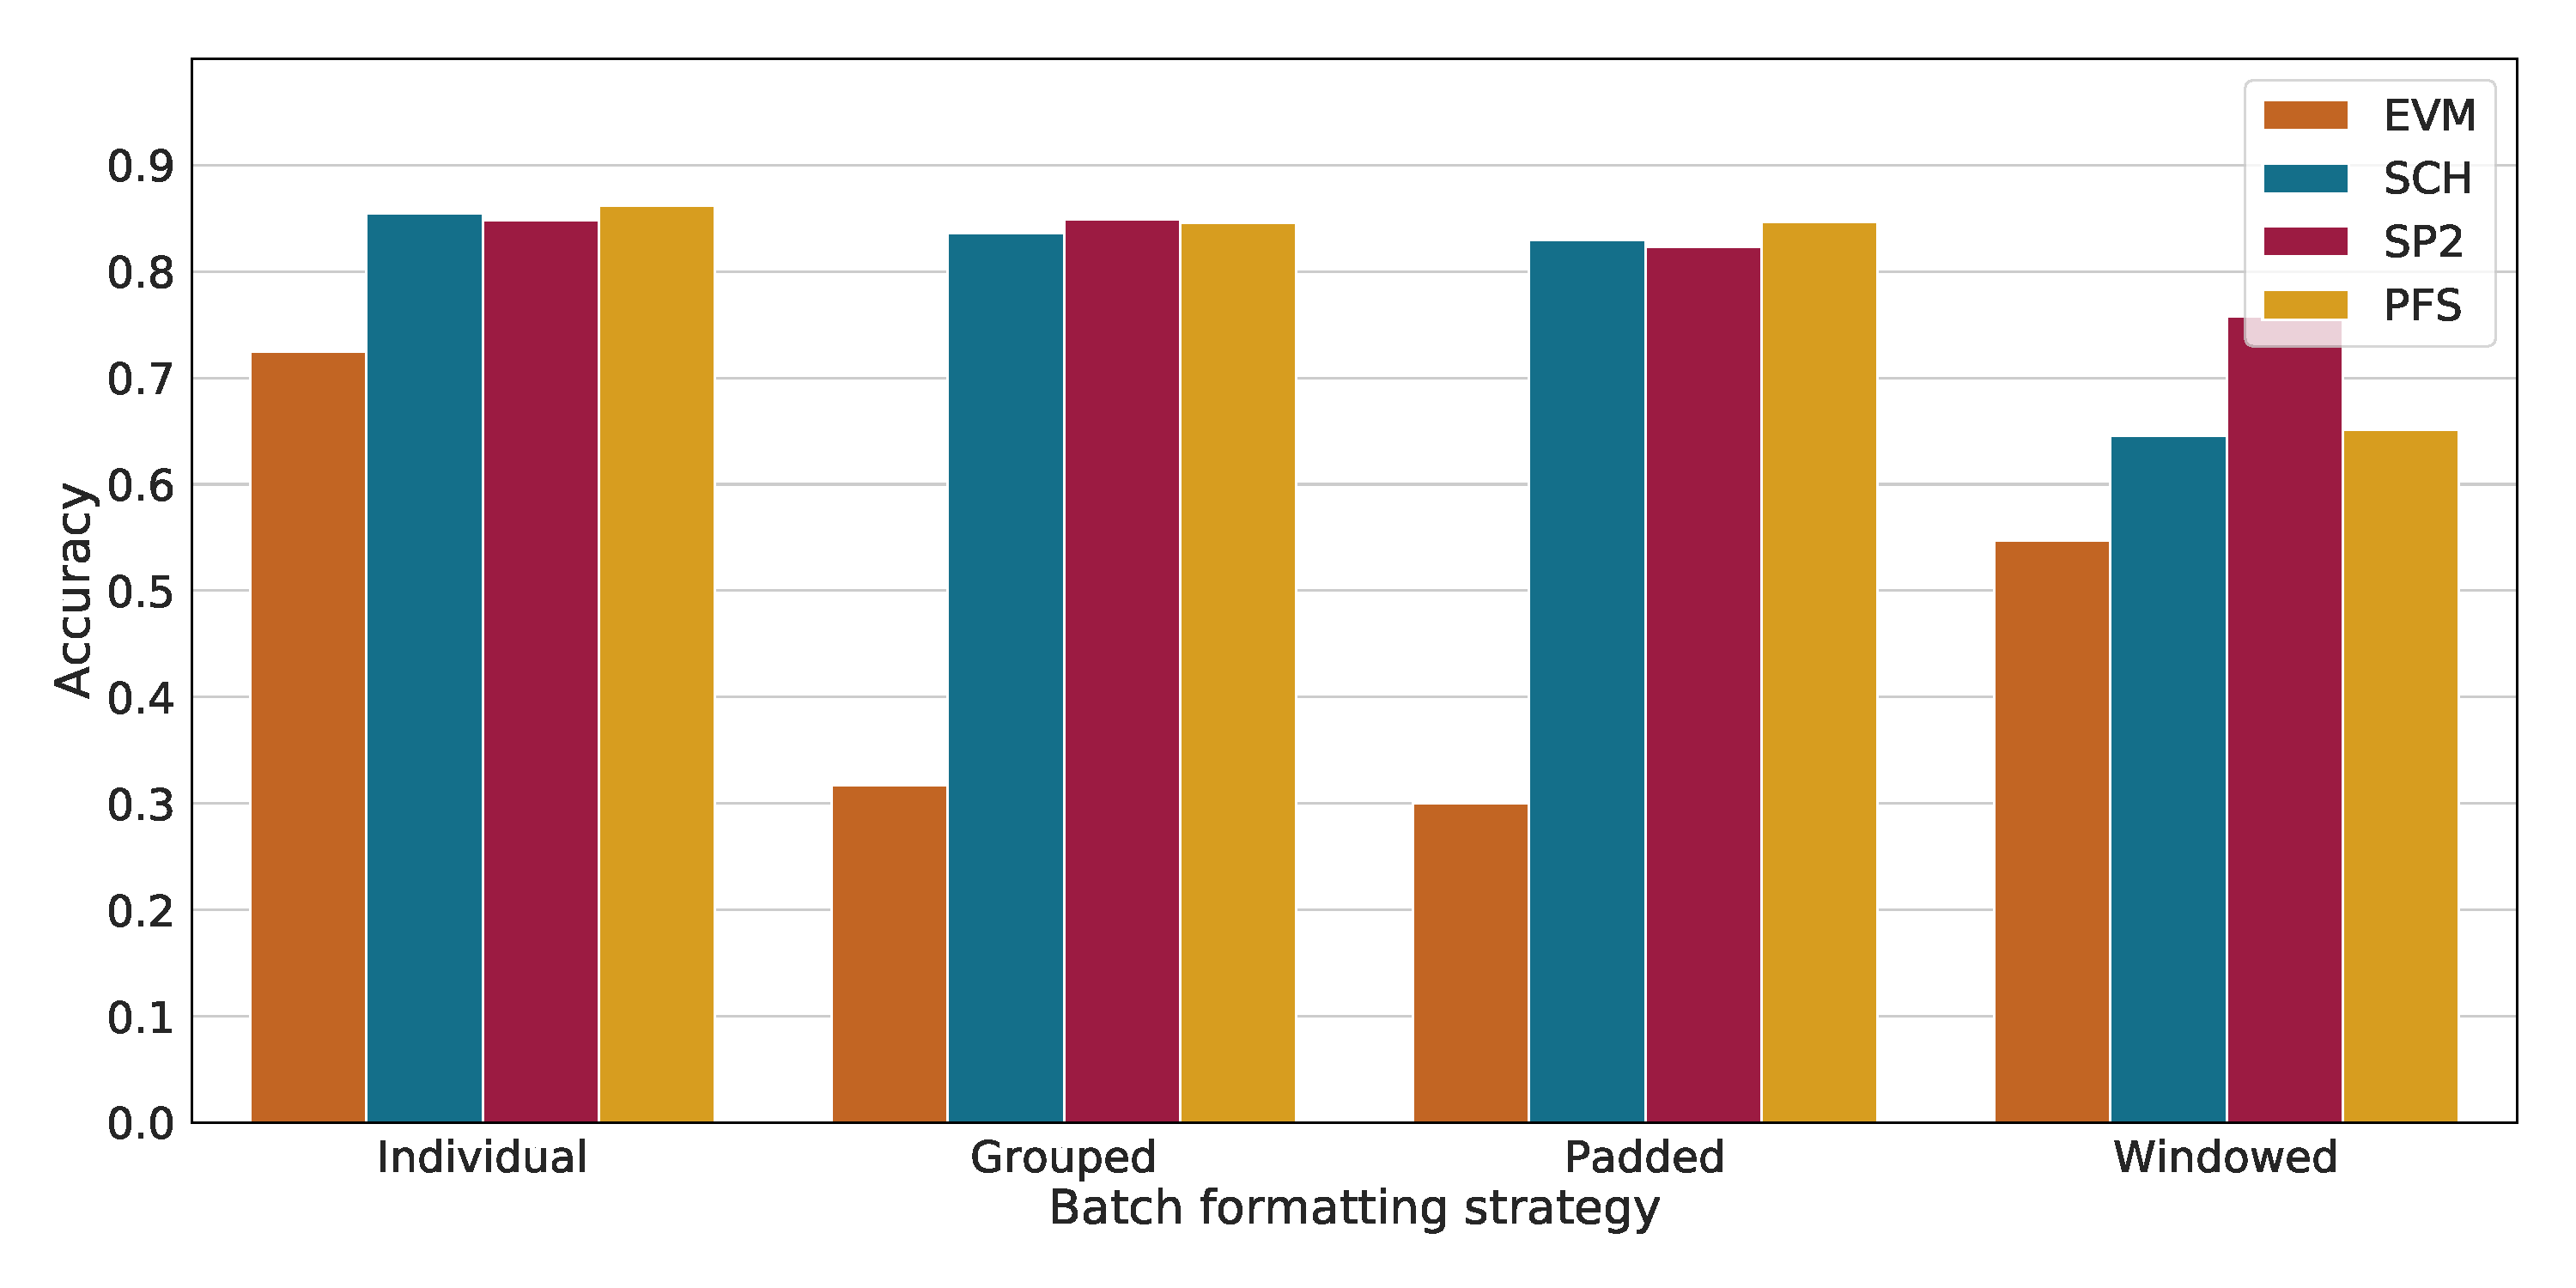
\includegraphics[width=\textwidth]{gfx/helpdesk/accuracies.pdf}
    \caption{Best accuracies on the validation set of HelpDesk}
    \label{fig:max-accuracies-helpdesk}
\end{figure}
\begin{figure}
    \centering
    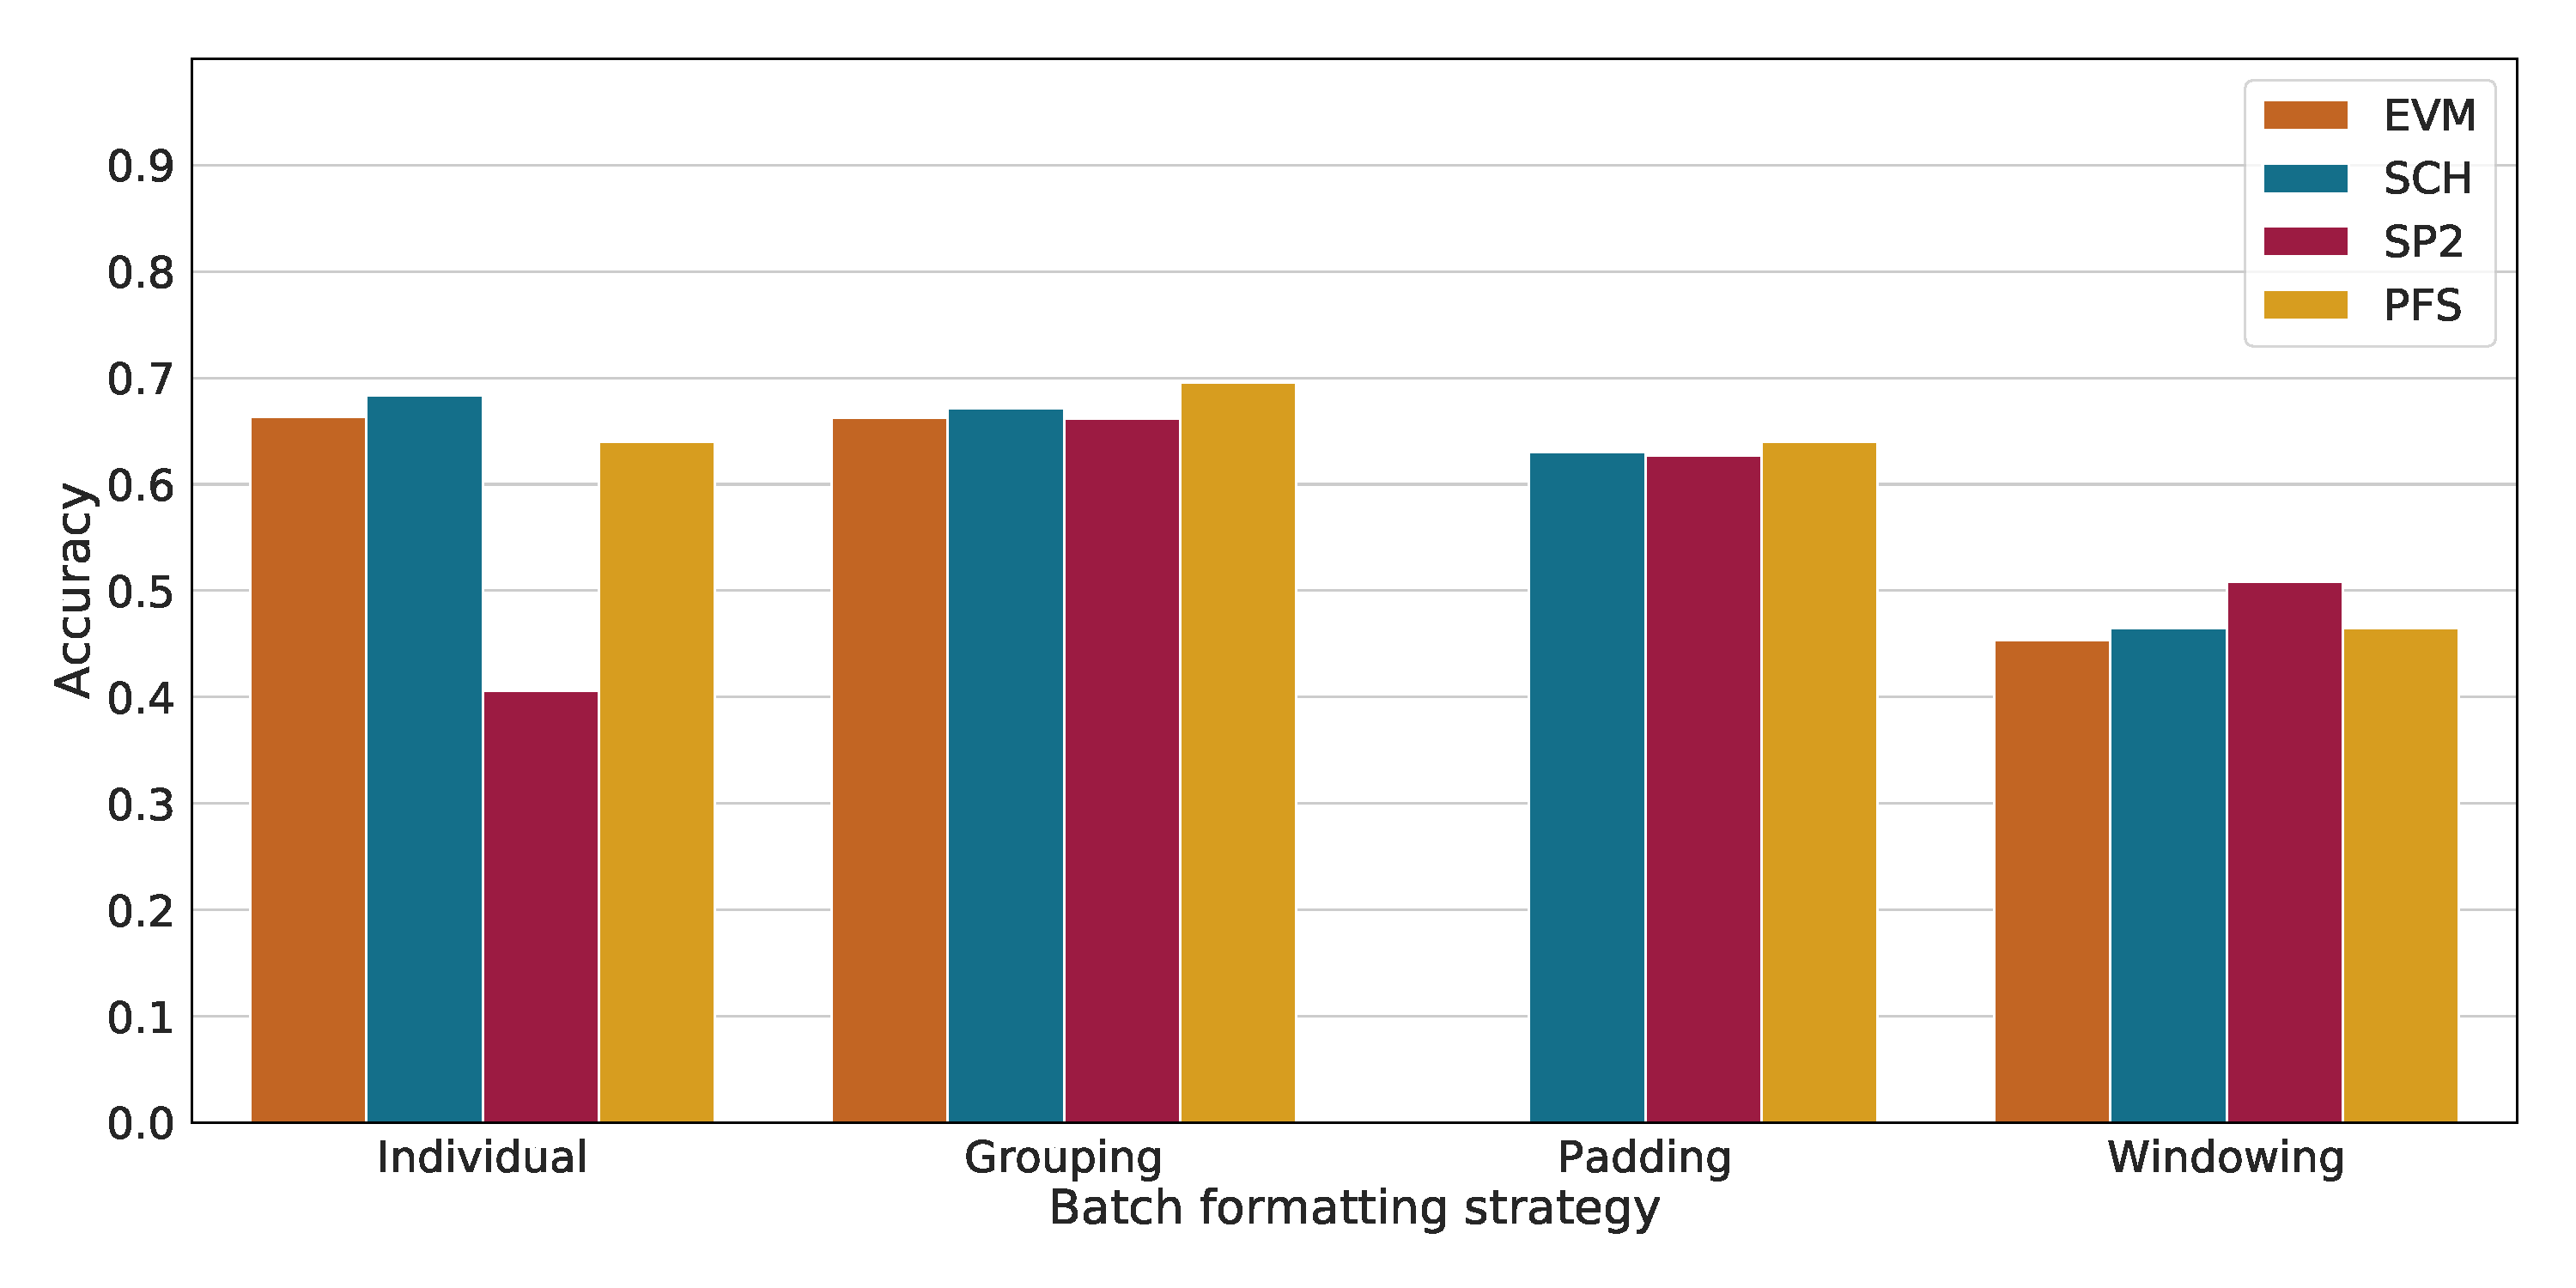
\includegraphics[width=\textwidth]{gfx/bpic2011/accuracies.pdf}
    \caption{Best accuracies on the validation set of BPIC11}
    \label{fig:max-accuracies-bpic2011}
\end{figure}
\begin{figure}
    \centering
    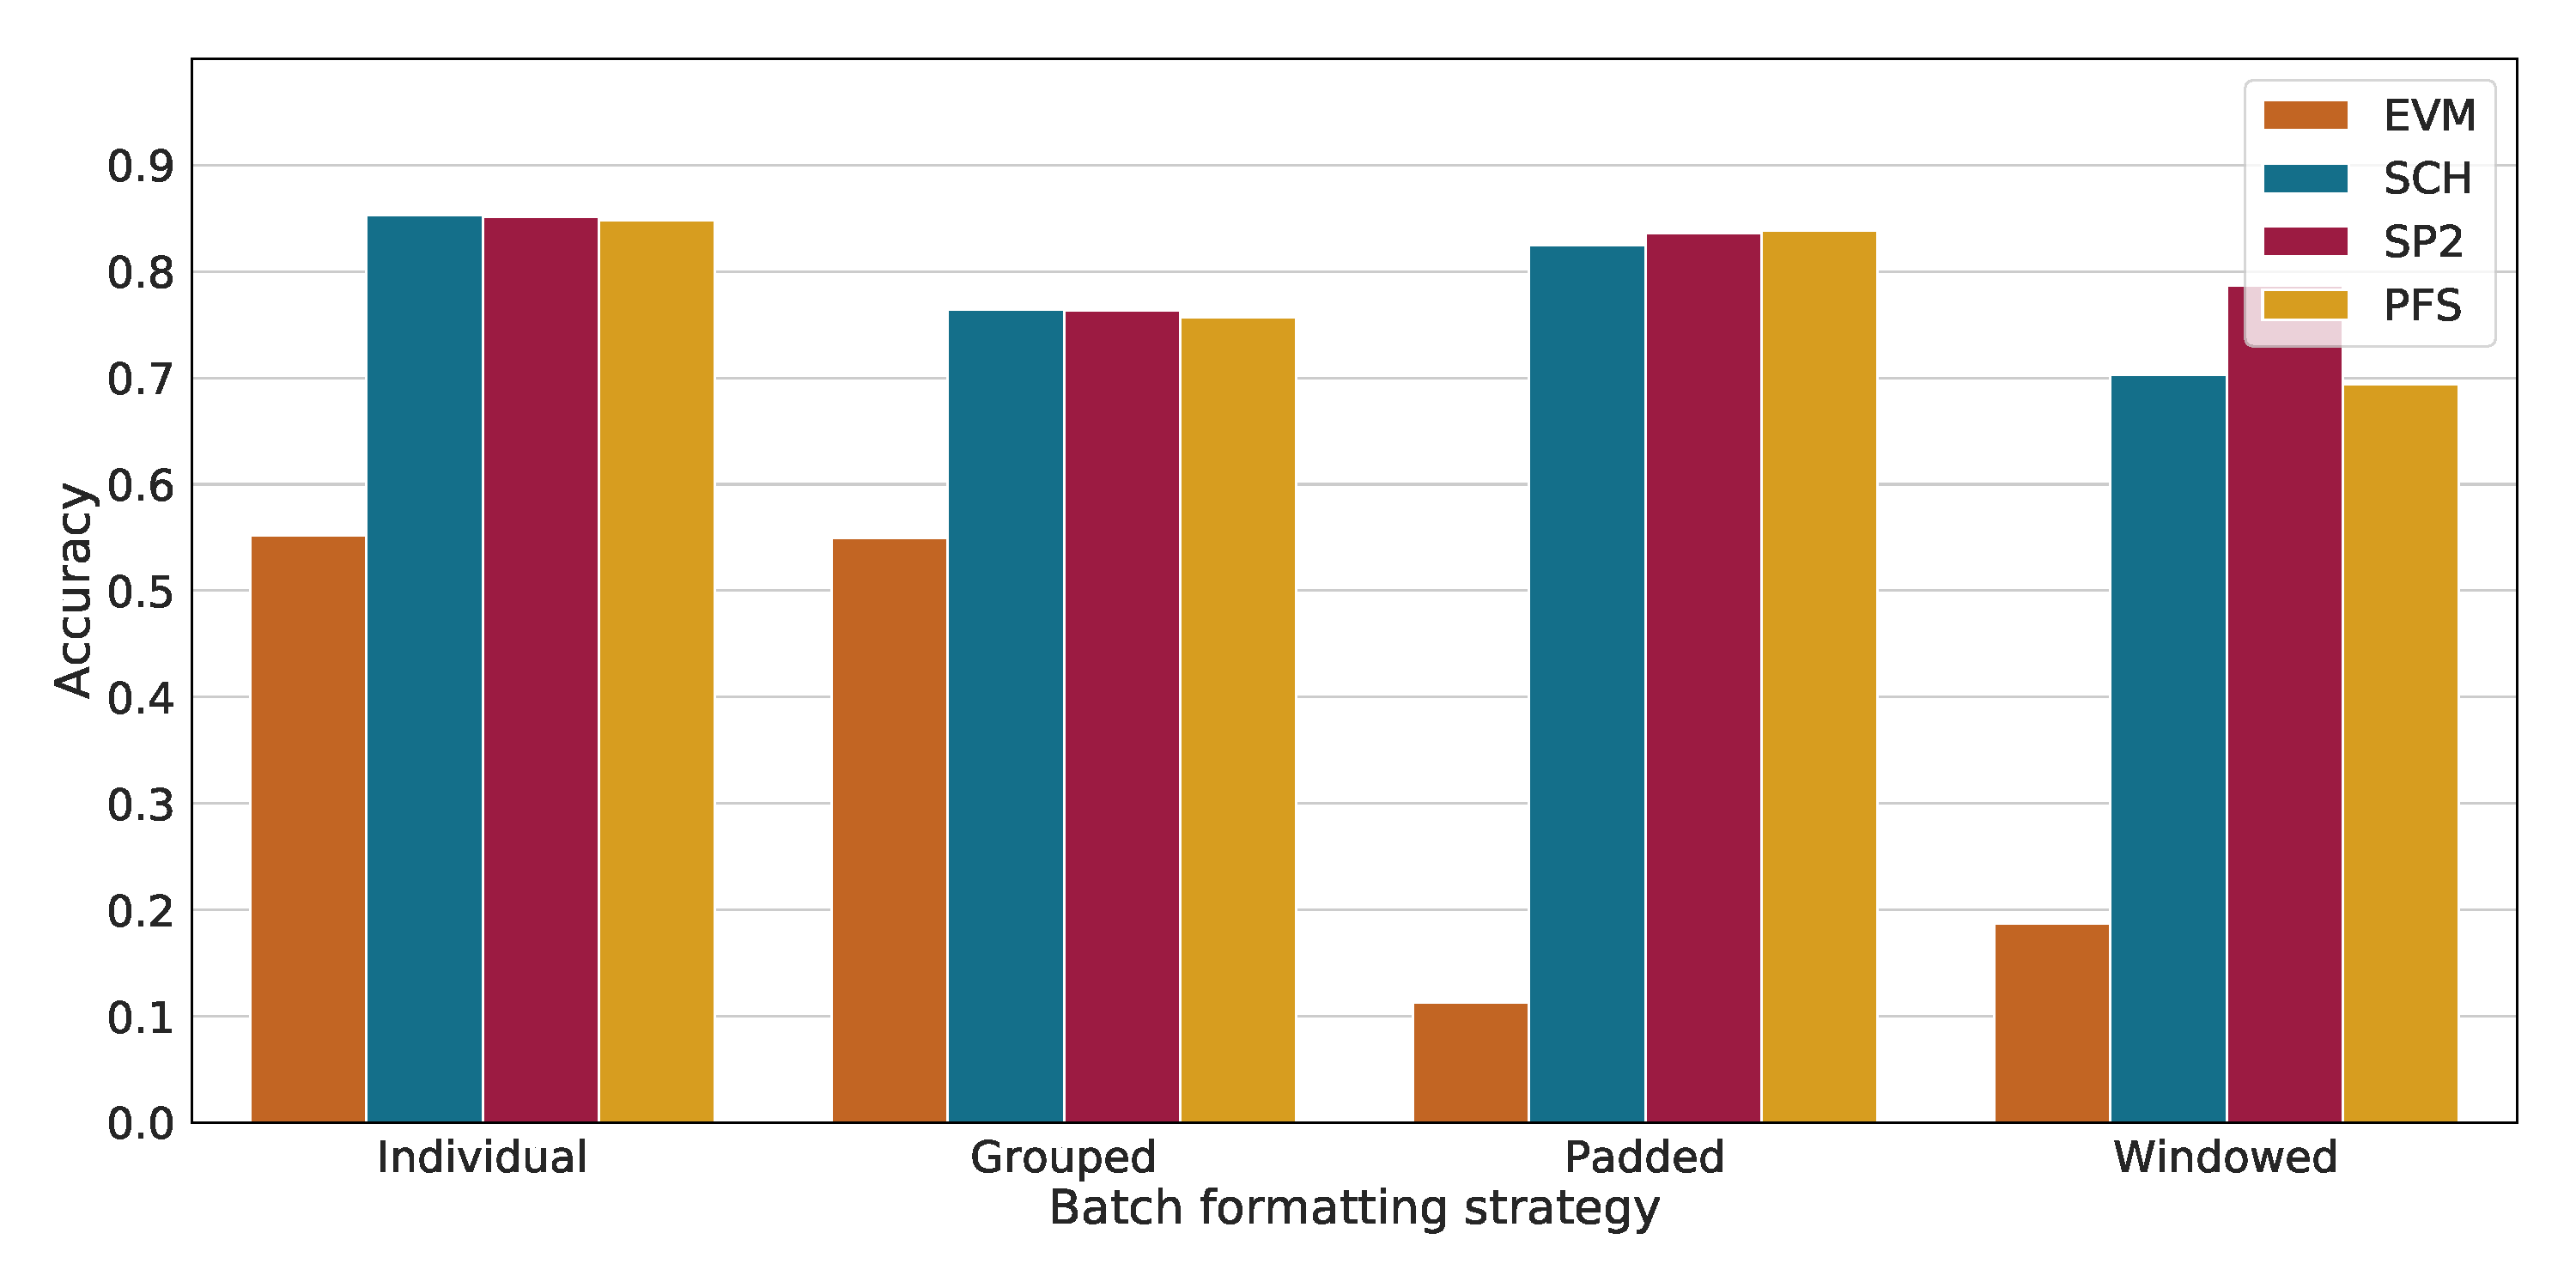
\includegraphics[width=\textwidth]{gfx/bpic2012/accuracies.pdf}
    \caption{Best accuracies on the validation set of BPIC12}
    \label{fig:max-accuracies-bpic2012}
\end{figure}
\begin{figure}
    \centering
    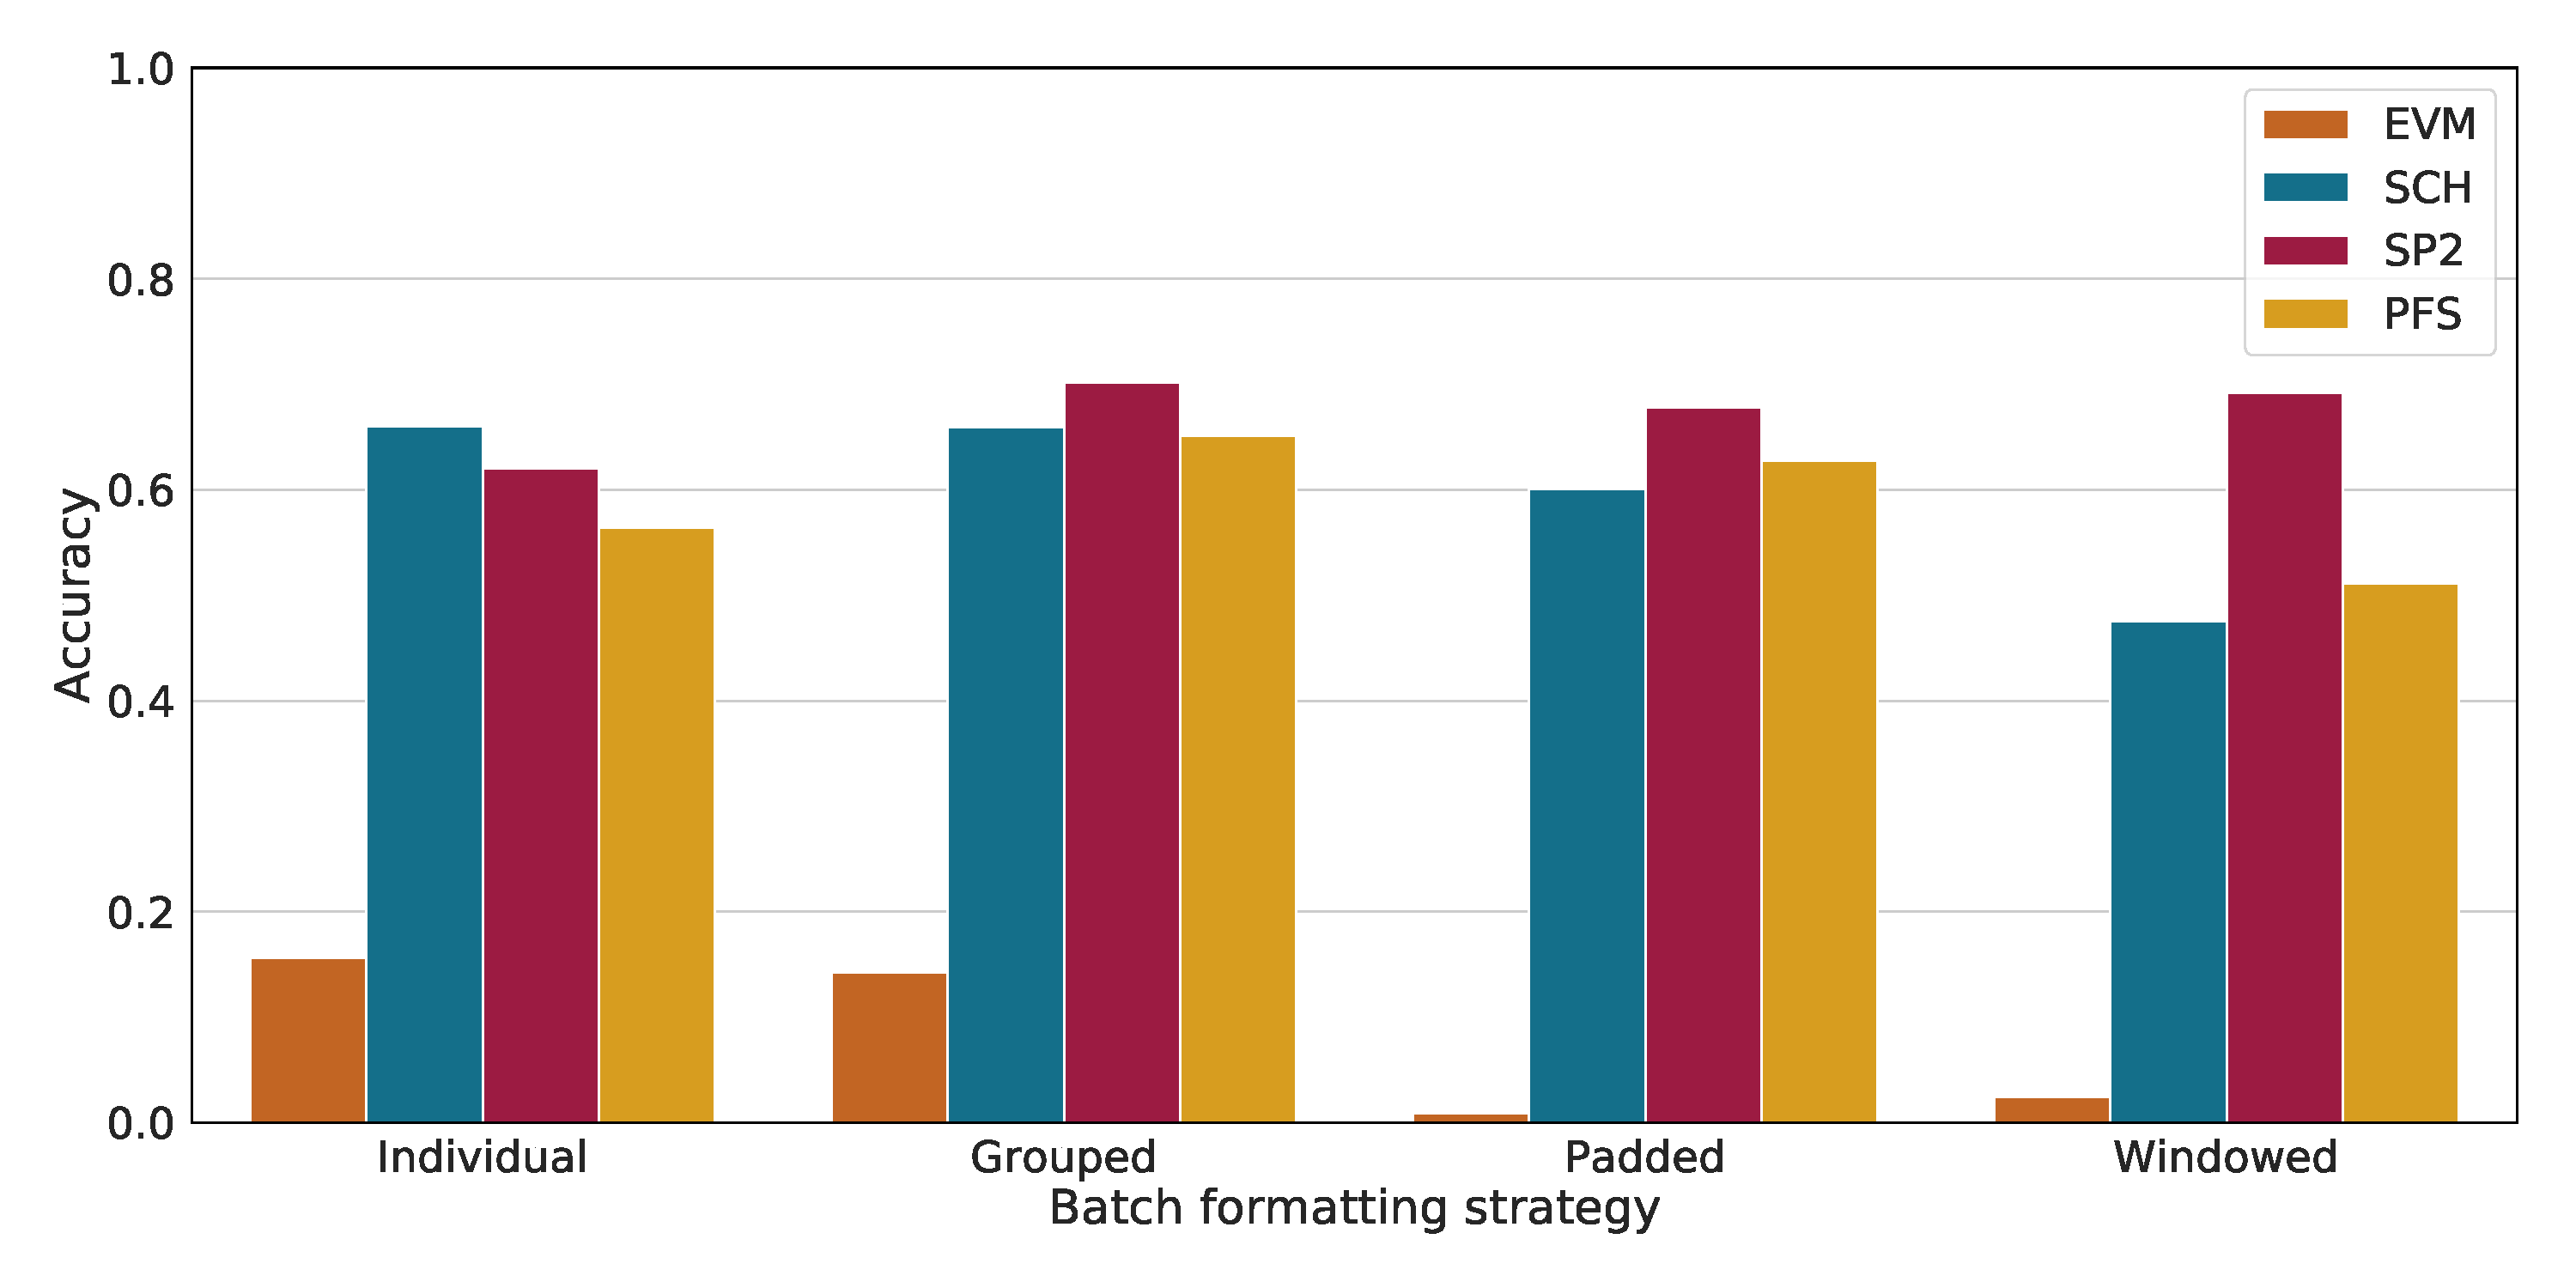
\includegraphics[width=\textwidth]{gfx/bpic2015_1/accuracies.pdf}
    \caption{Best accuracies on the validation set of BPIC15-1}
    \label{fig:max-accuracies-bpic2015-1}
\end{figure}
\begin{figure}
    \centering
    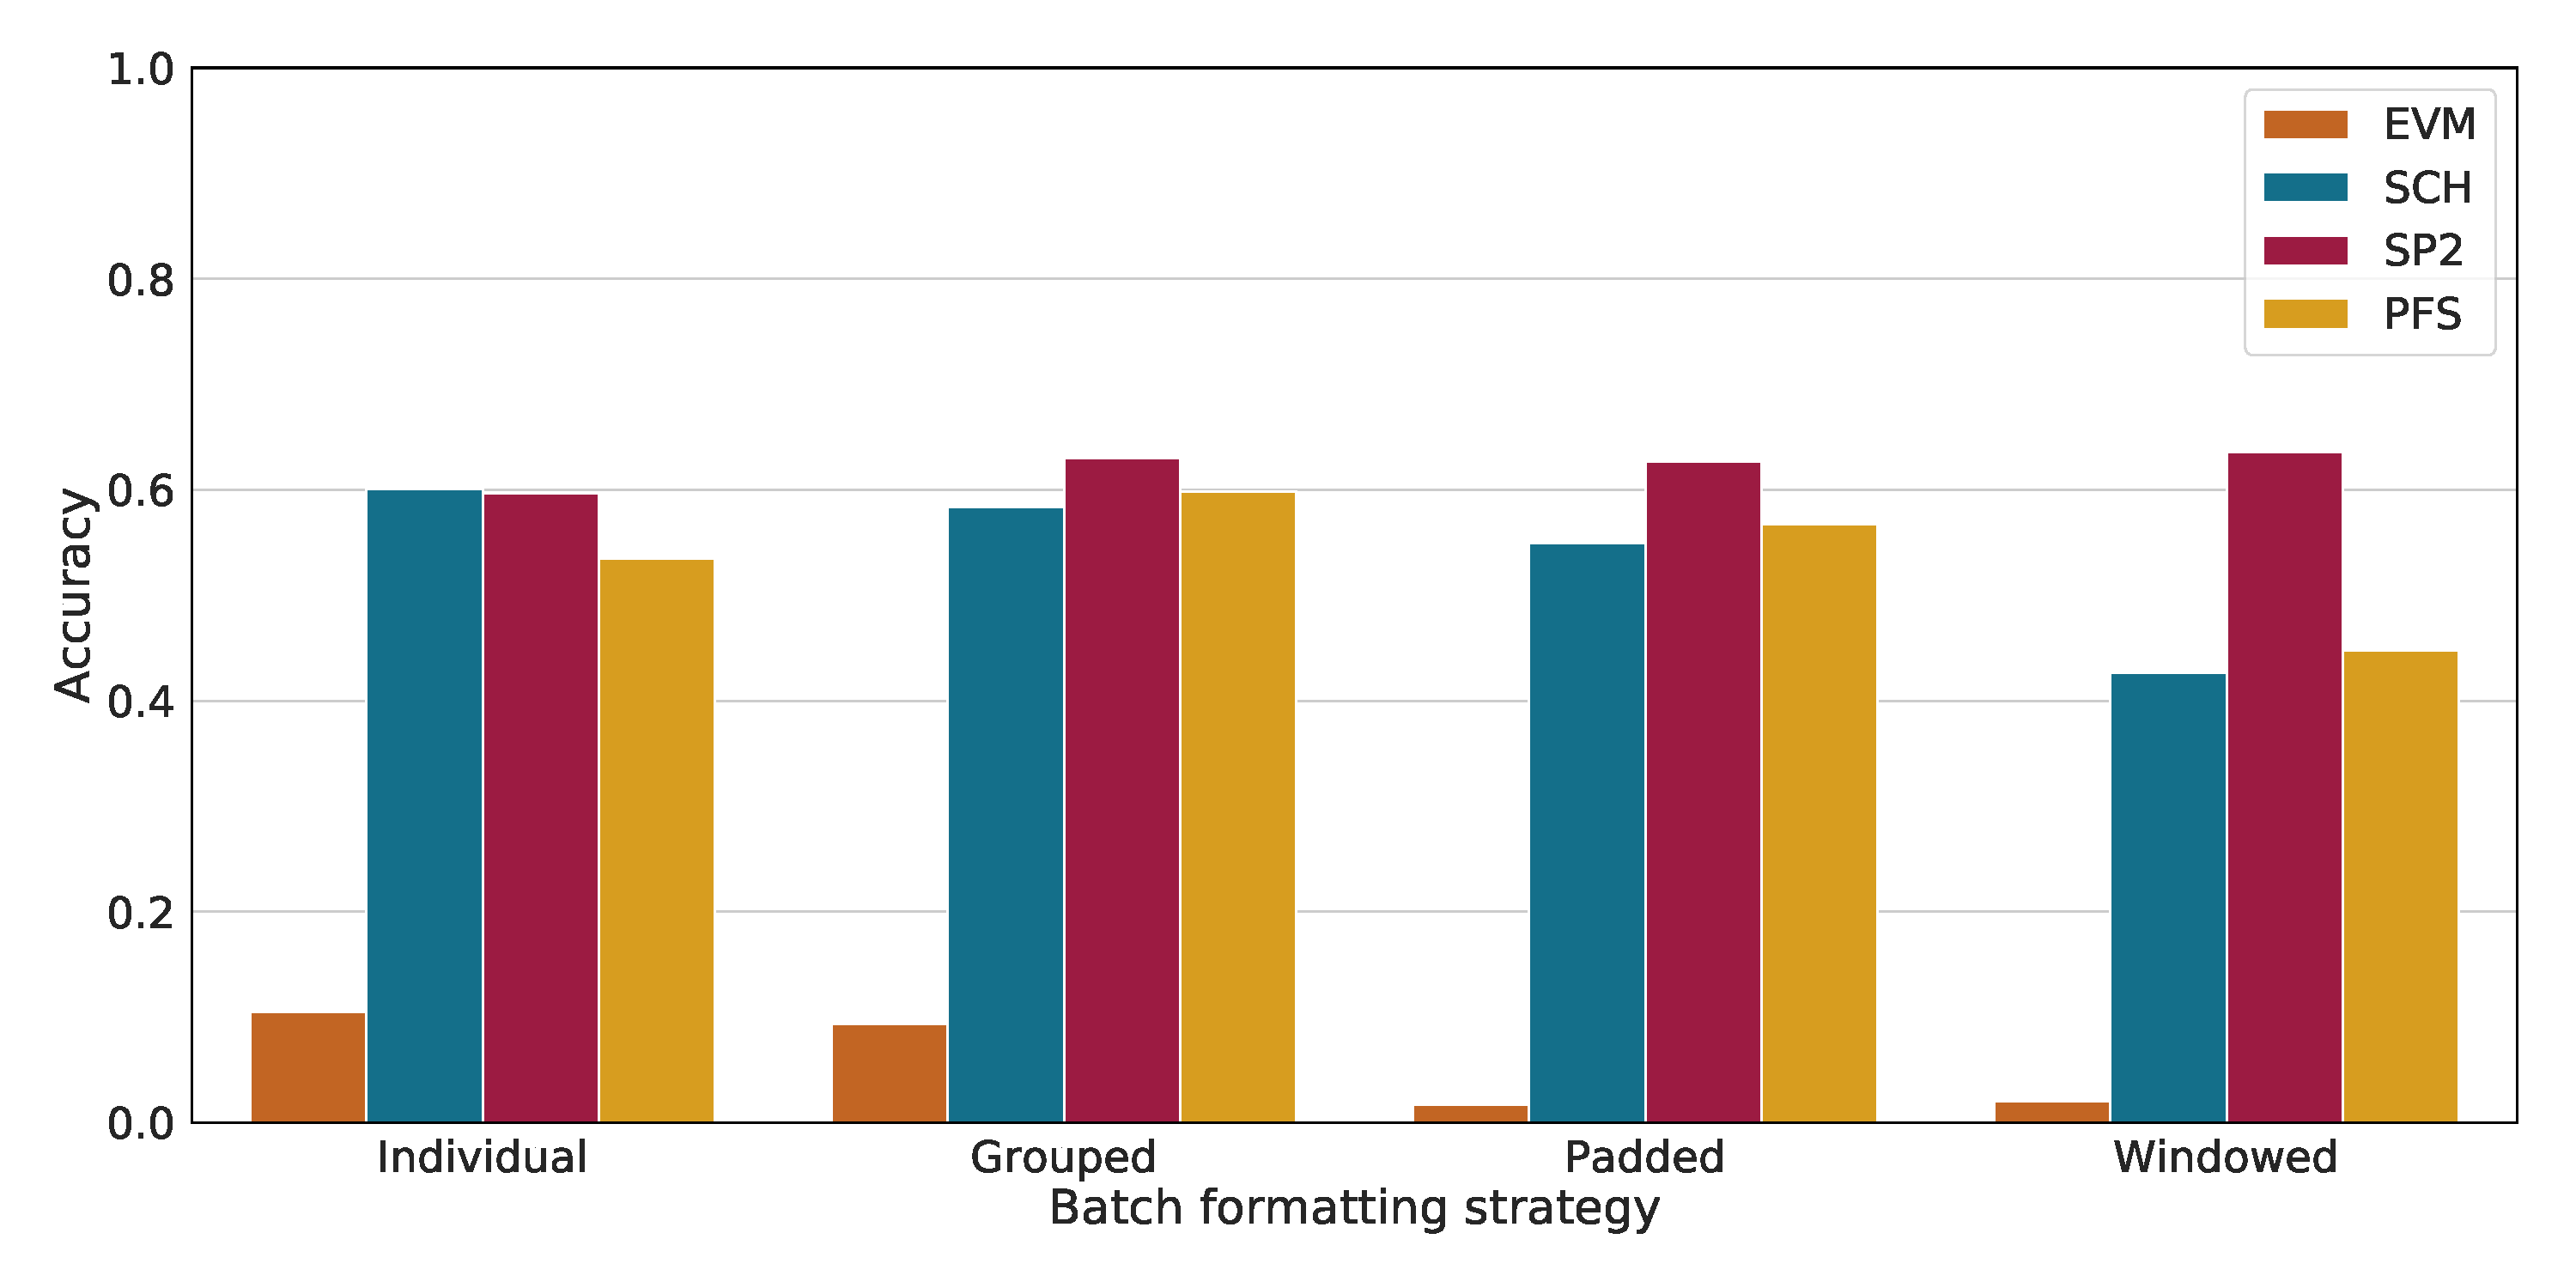
\includegraphics[width=\textwidth]{gfx/bpic2015_2/accuracies.pdf}
    \caption{Best accuracies on the validation set of BPIC15-2}
    \label{fig:max-accuracies-bpic2015-2}
\end{figure}
\begin{figure}
    \centering
    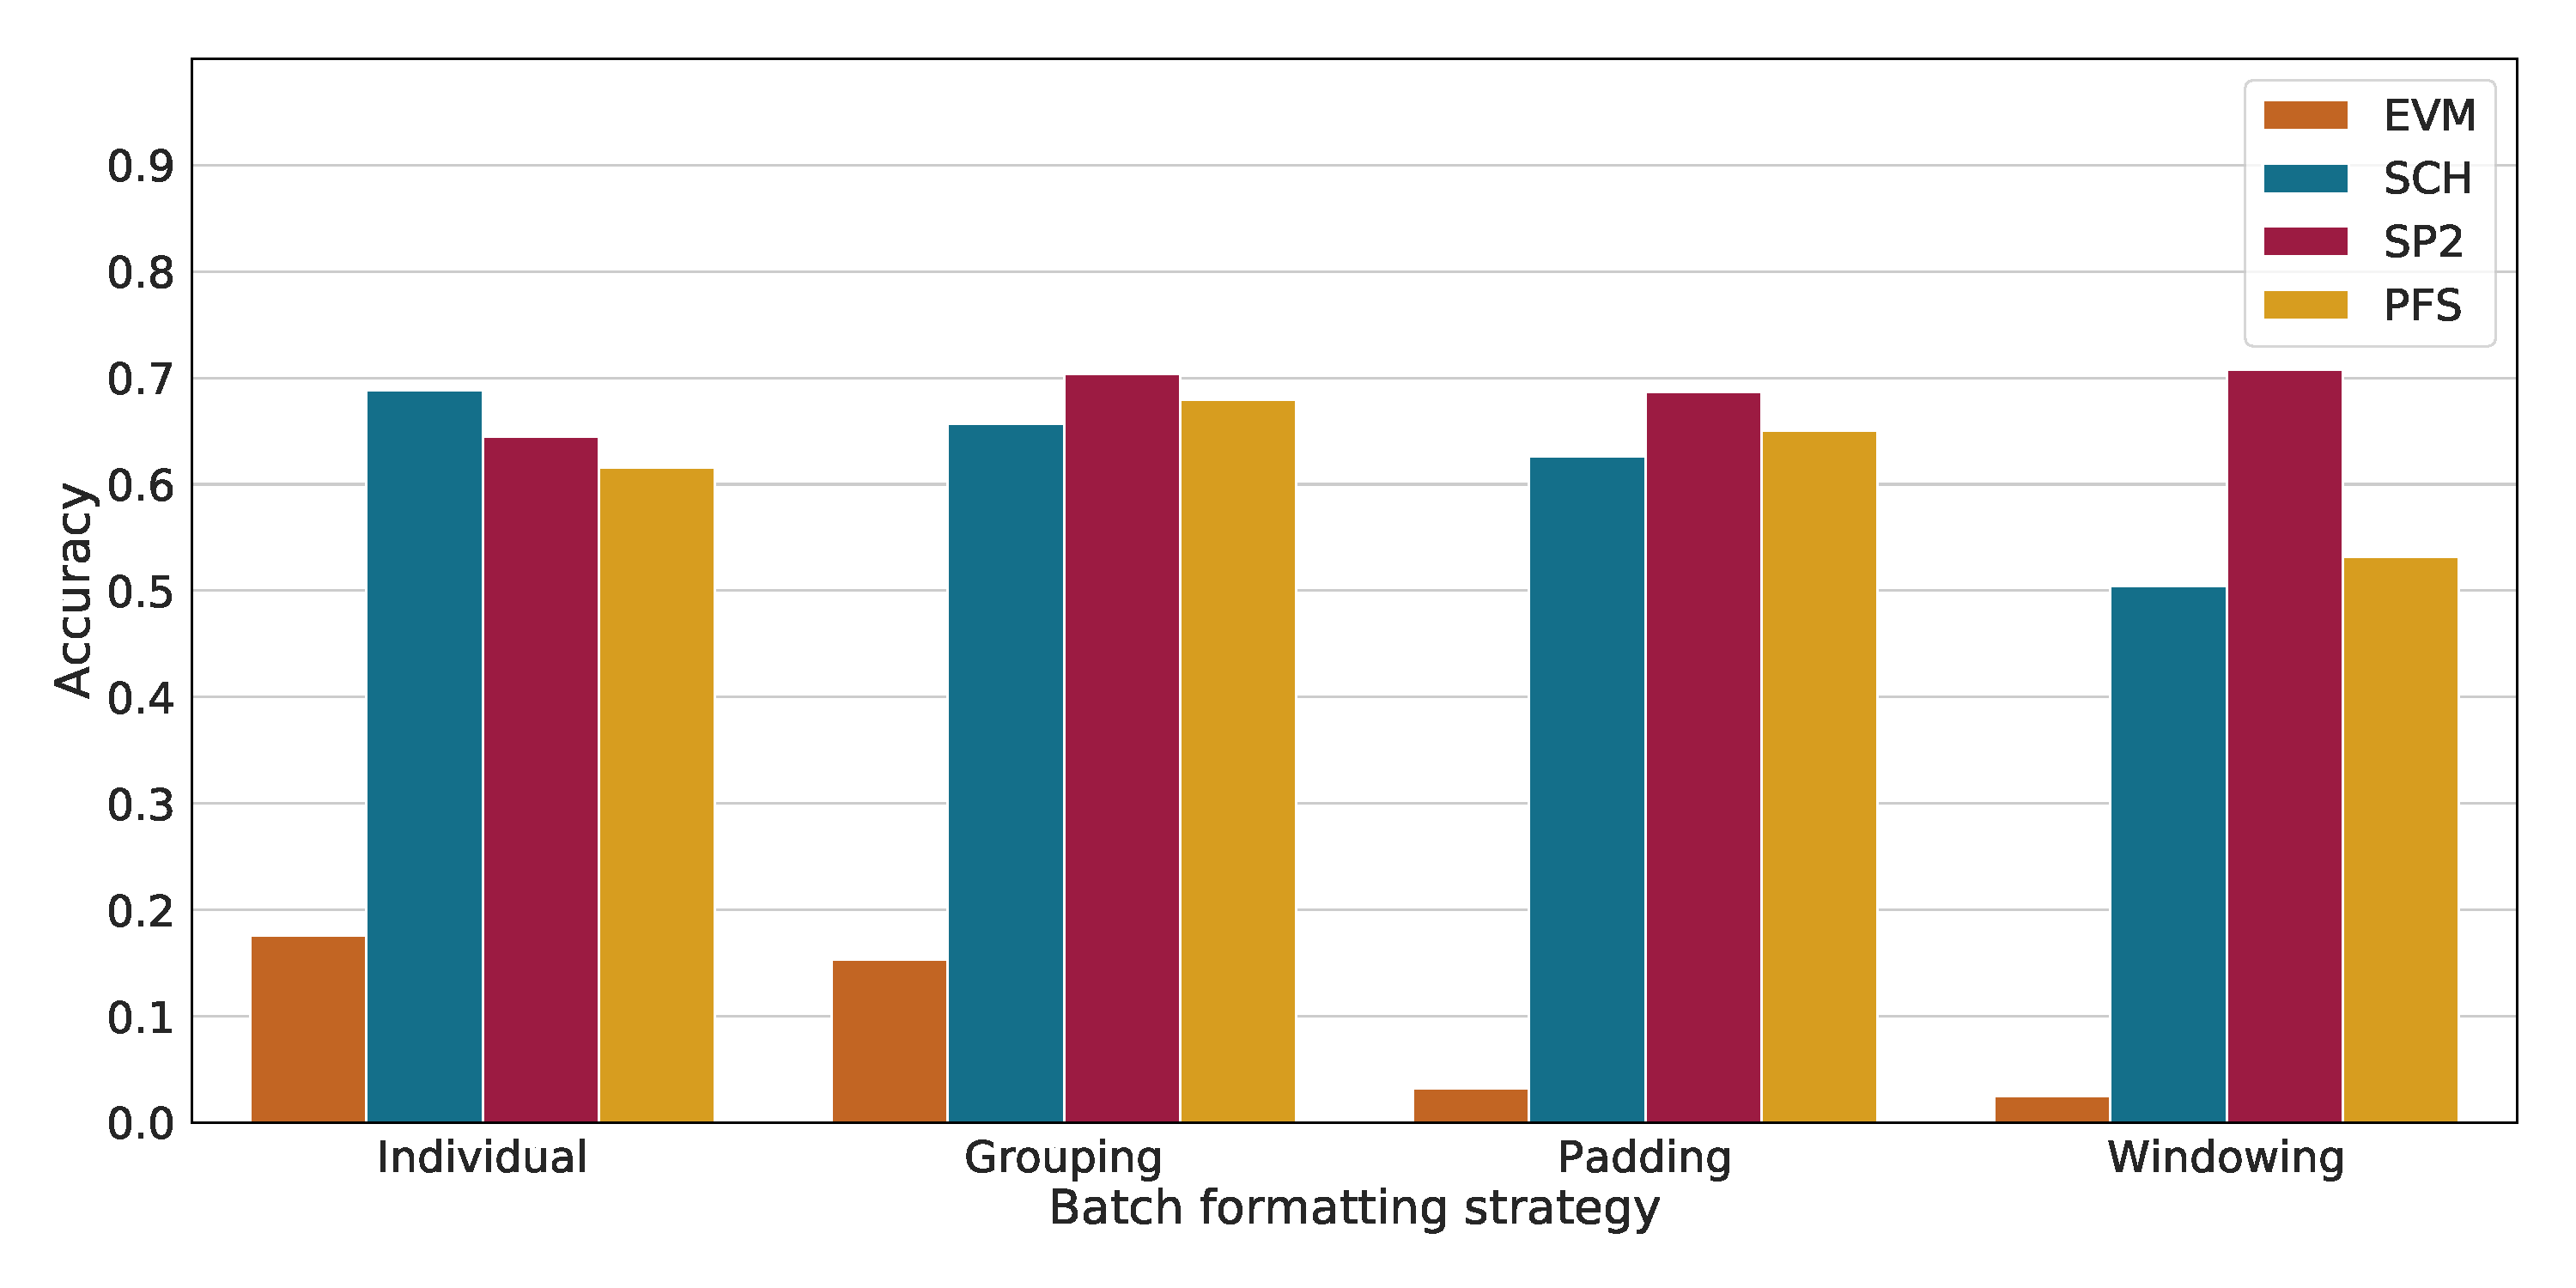
\includegraphics[width=\textwidth]{gfx/bpic2015_3/accuracies.pdf}
    \caption{Best accuracies on the validation set of BPIC15-3}
    \label{fig:max-accuracies-bpic2015-3}
\end{figure}
\begin{figure}
    \centering
    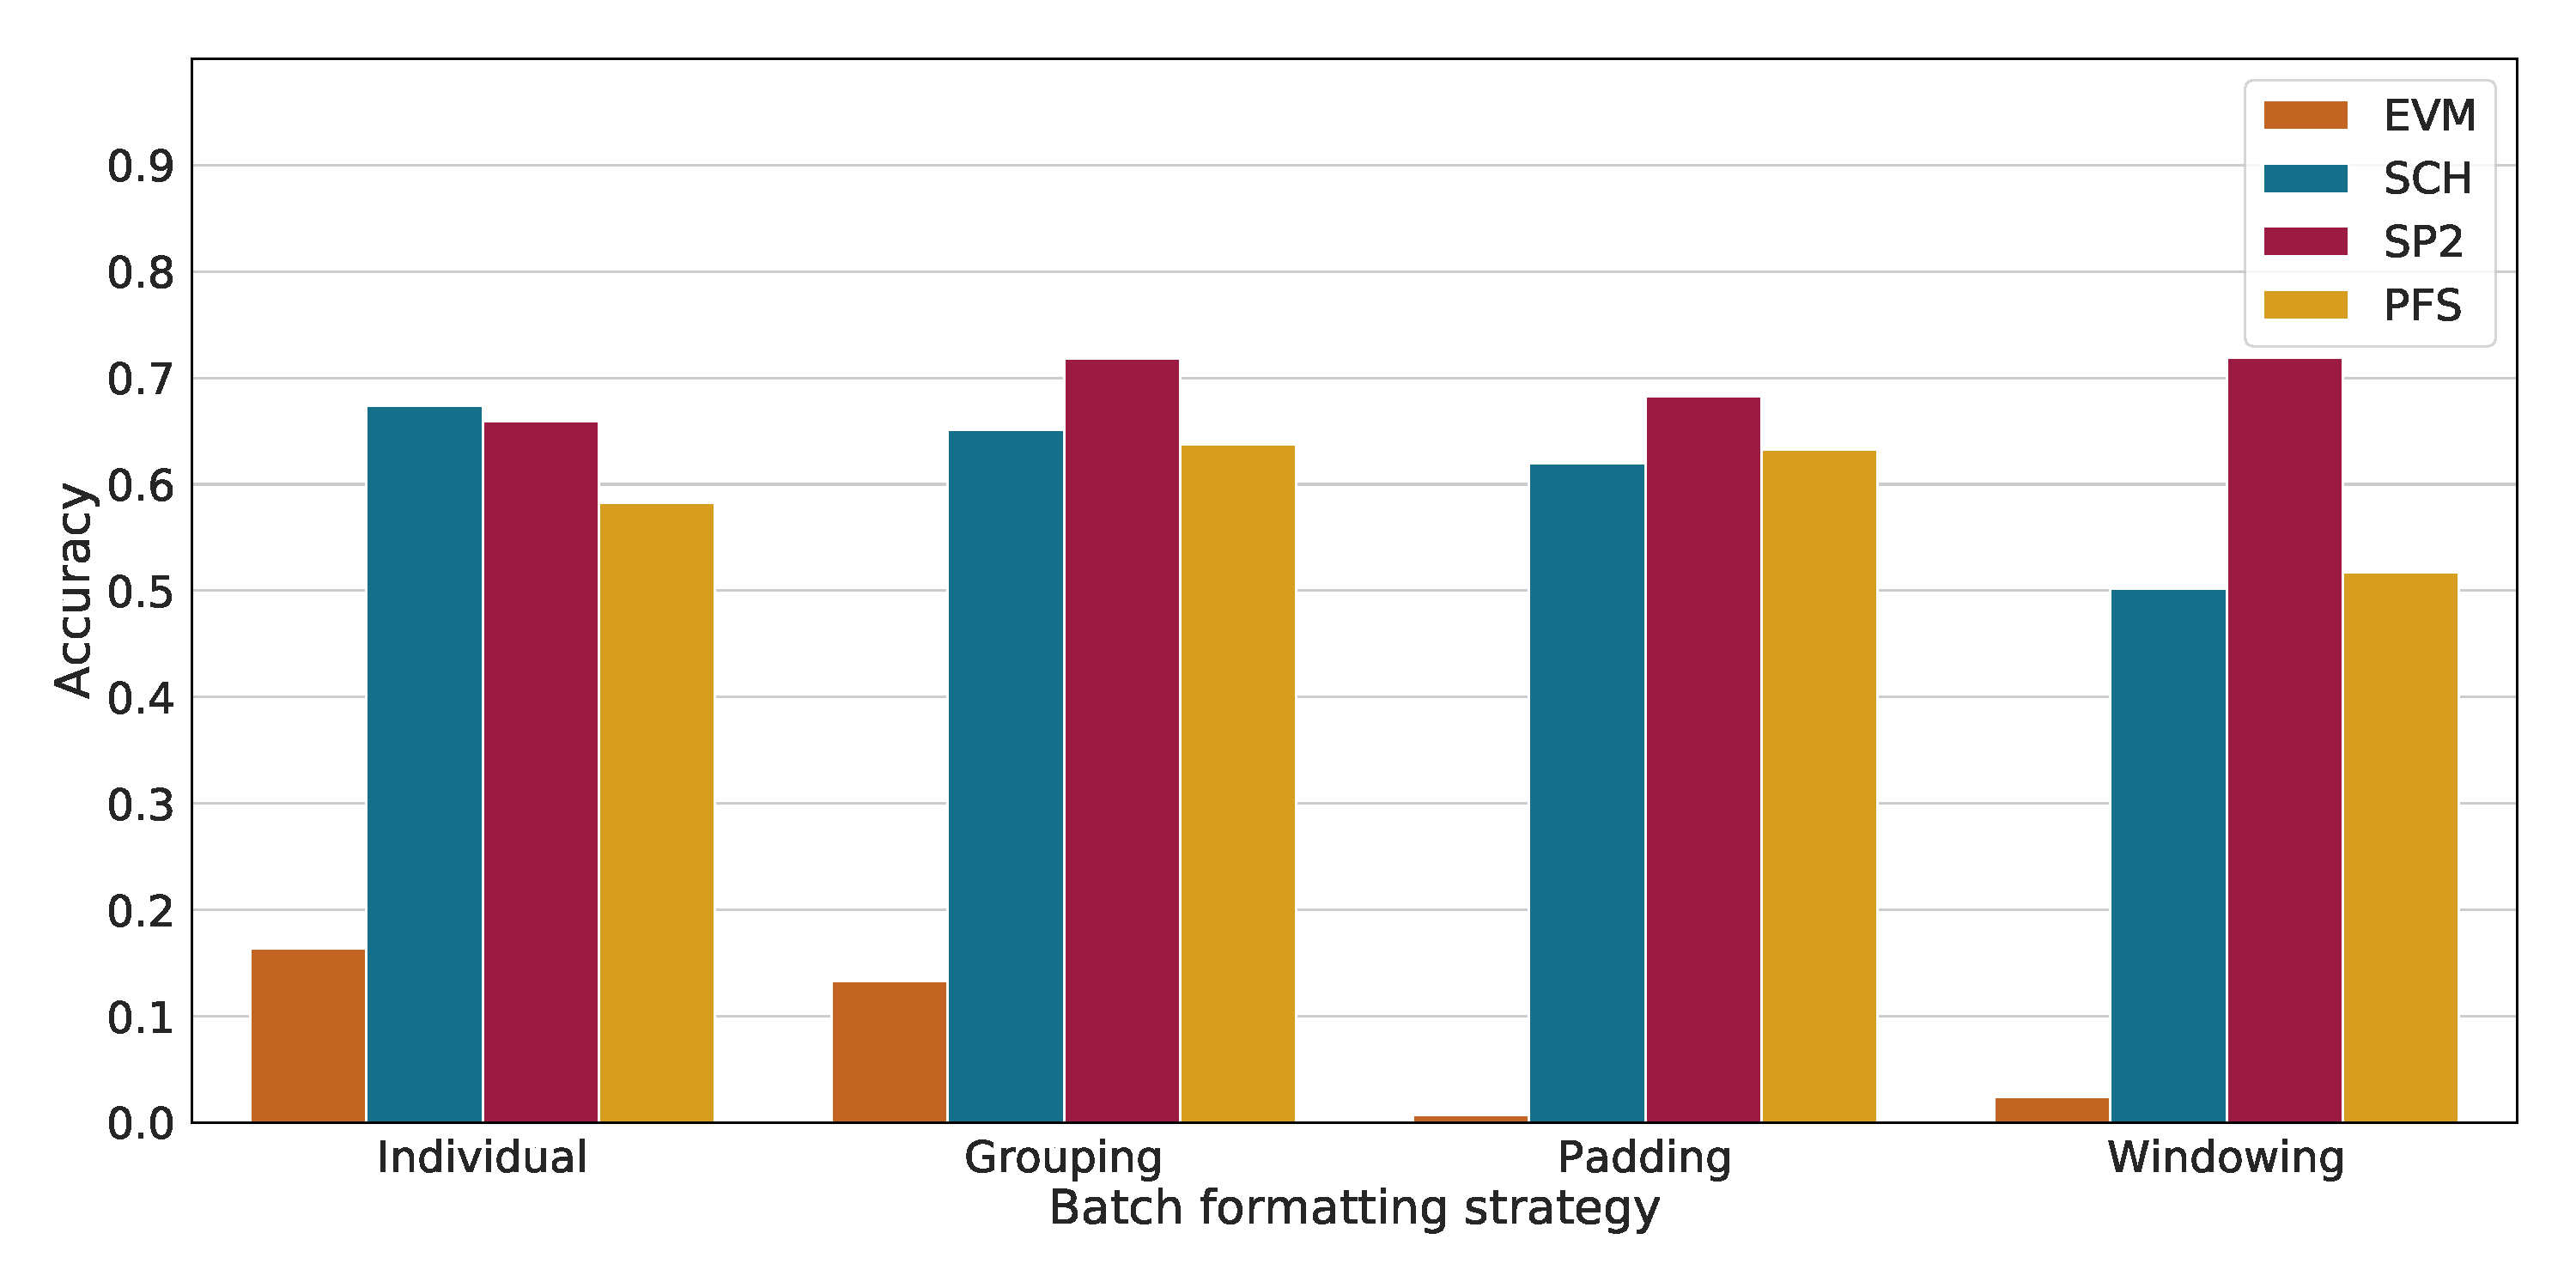
\includegraphics[width=\textwidth]{gfx/bpic2015_4/accuracies.pdf}
    \caption{Best accuracies on the validation set of BPIC15-4}
    \label{fig:max-accuracies-bpic2015-4}
\end{figure}
\begin{figure}
    \centering
    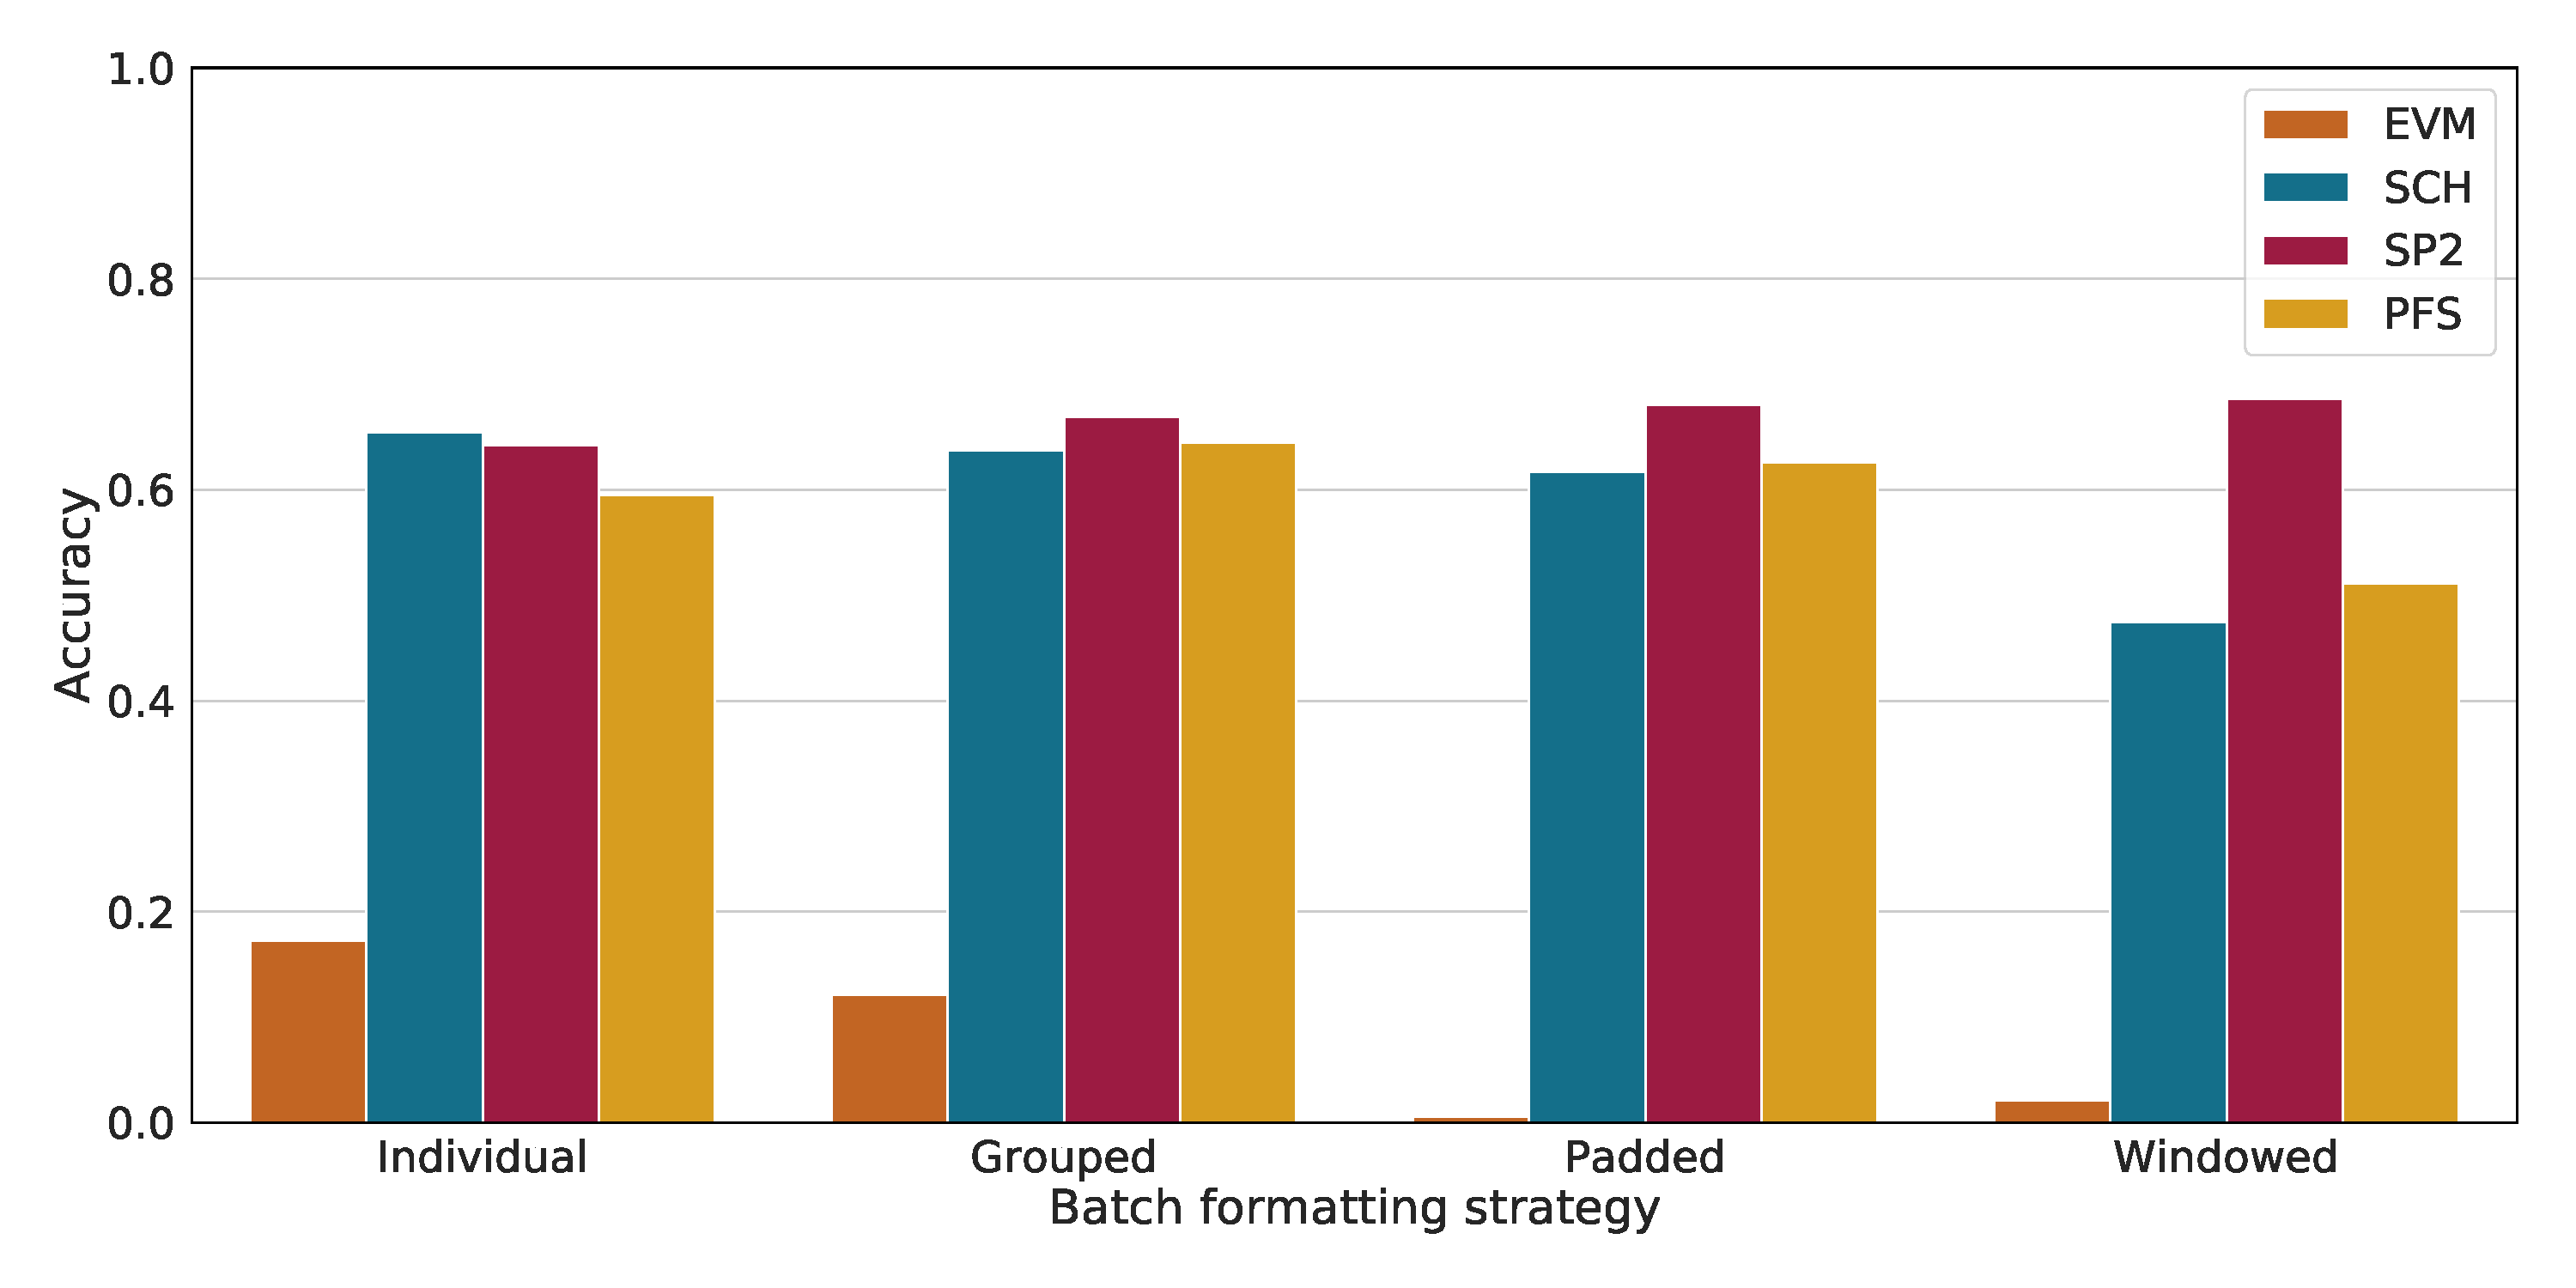
\includegraphics[width=\textwidth]{gfx/bpic2015_5/accuracies.pdf}
    \caption{Best accuracies on the validation set of BPIC15-5}
    \label{fig:max-accuracies-bpic2015-5}
\end{figure}
\begin{table}
\centering
\begin{tabular}{l|rrrr}
Dataset  &  Individual &   Grouped &    Padded &  Windowed \\
\midrule
HelpDesk &    0.85     &  0.84     &  0.83     &  0.68     \\
BPIC11   &    0.576    &  0.676    &  0.632    &  0.479    \\
BPIC12   &    0.850    &  0.761    &  0.833    &  0.728    \\
BPIC15-1 &    0.614    &  0.670    &  0.635    &  0.559    \\
BPIC15-2 &    0.577    &  0.604    &  0.581    &  0.503    \\
BPIC15-3 &    0.649    &  0.680    &  0.654    &  0.581    \\
BPIC15-4 &    0.638    &  0.668    &  0.645    &  0.579    \\
BPIC15-5 &    0.630    &  0.650    &  0.640    &  0.557    \\
\end{tabular}
\caption[Grouping strategy leads to best mean accuracies]{Accuracy means across the top accuracies of the SCH, SP2 and PFS models. The grouping strategy is generally the highest}
\label{tab:strategy-top-accuracies}
\end{table}
\FloatBarrier

\section{Training time}\label{sec:eval:training-time}
The training time that a model requires for an epoch is important to gauge the efficiency of its training process. The batch size has a direct effect on the required time since it corresponds to the number of weight adjustments that need to be calculated. \autoref{fig:helpdesk-training-timings} to \autoref{fig:BPIC15-5-training-timings} illustrate the mean time required for training a model for an epoch, grouped by batching strategy. We go over the training times per batching strategy and explain the results.

Unsurprisingly, the individual batching strategy leads to the longest times overall. \autoref{tab:dataset-characteristics} reveals that this strategy leads to hundreds of weight adjustments per epoch.

The grouped batching strategy leads to significant reductions in training times, depending on how diverse the trace lengths are. \autoref{tab:dataset-characteristics} explains why the reduction is not as prominent with BPIC11: It exhibits up to 1814 different lengths, while the other datasets only exhibit $5\%$ to $10\%$ of this number.

With the padded strategy, it is possible to overcome the limitations imposed by trace lengths and construct batches out of any number of traces. This makes it easier to optimize the batch size, which can lead to faster training times.
%That it does not always lead to better accuracies was shown in the previous section, as, e.g. this strategy incurs a loss of samples on BPIC11.

Finally, the windowing strategy is the fastest.
It produces a constant number of timesteps and allows for arbitrary batch sizes.
The low number of timesteps additionally reduces the amount of calculation that needs to be done.

\begin{figure}
    \centering
    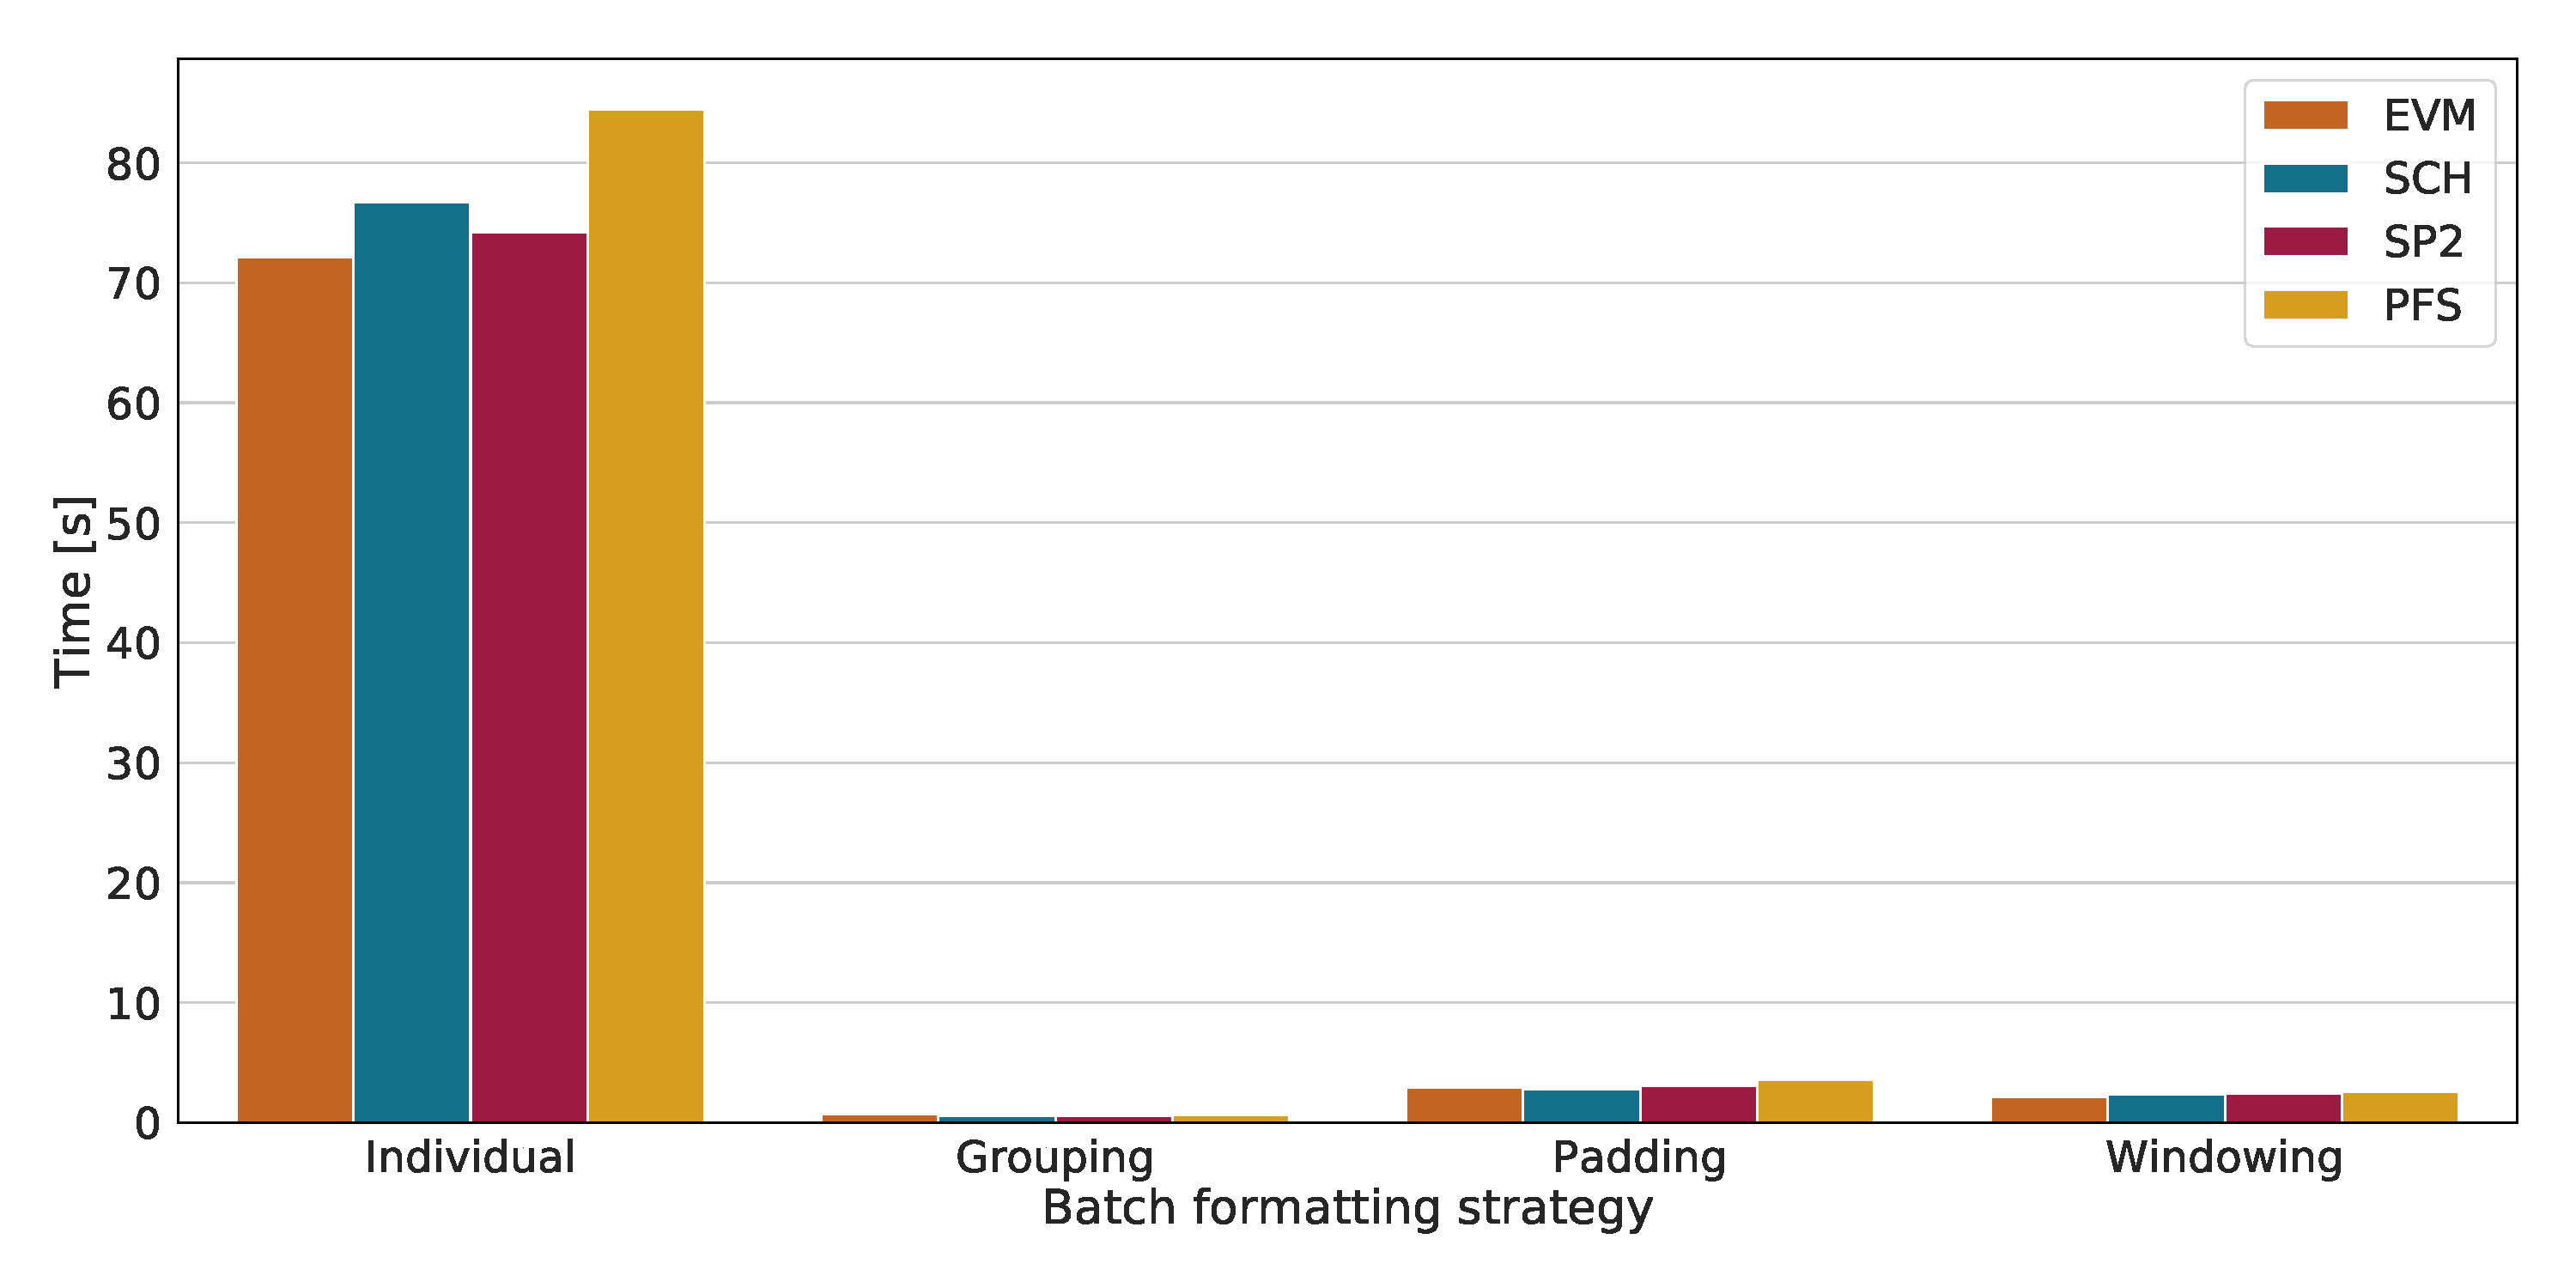
\includegraphics[width=\textwidth]{gfx/helpdesk/train_timings.pdf}
    \caption{Training times measured on HelpDesk}
    \label{fig:helpdesk-training-timings}
\end{figure}
\begin{figure}
    \centering
    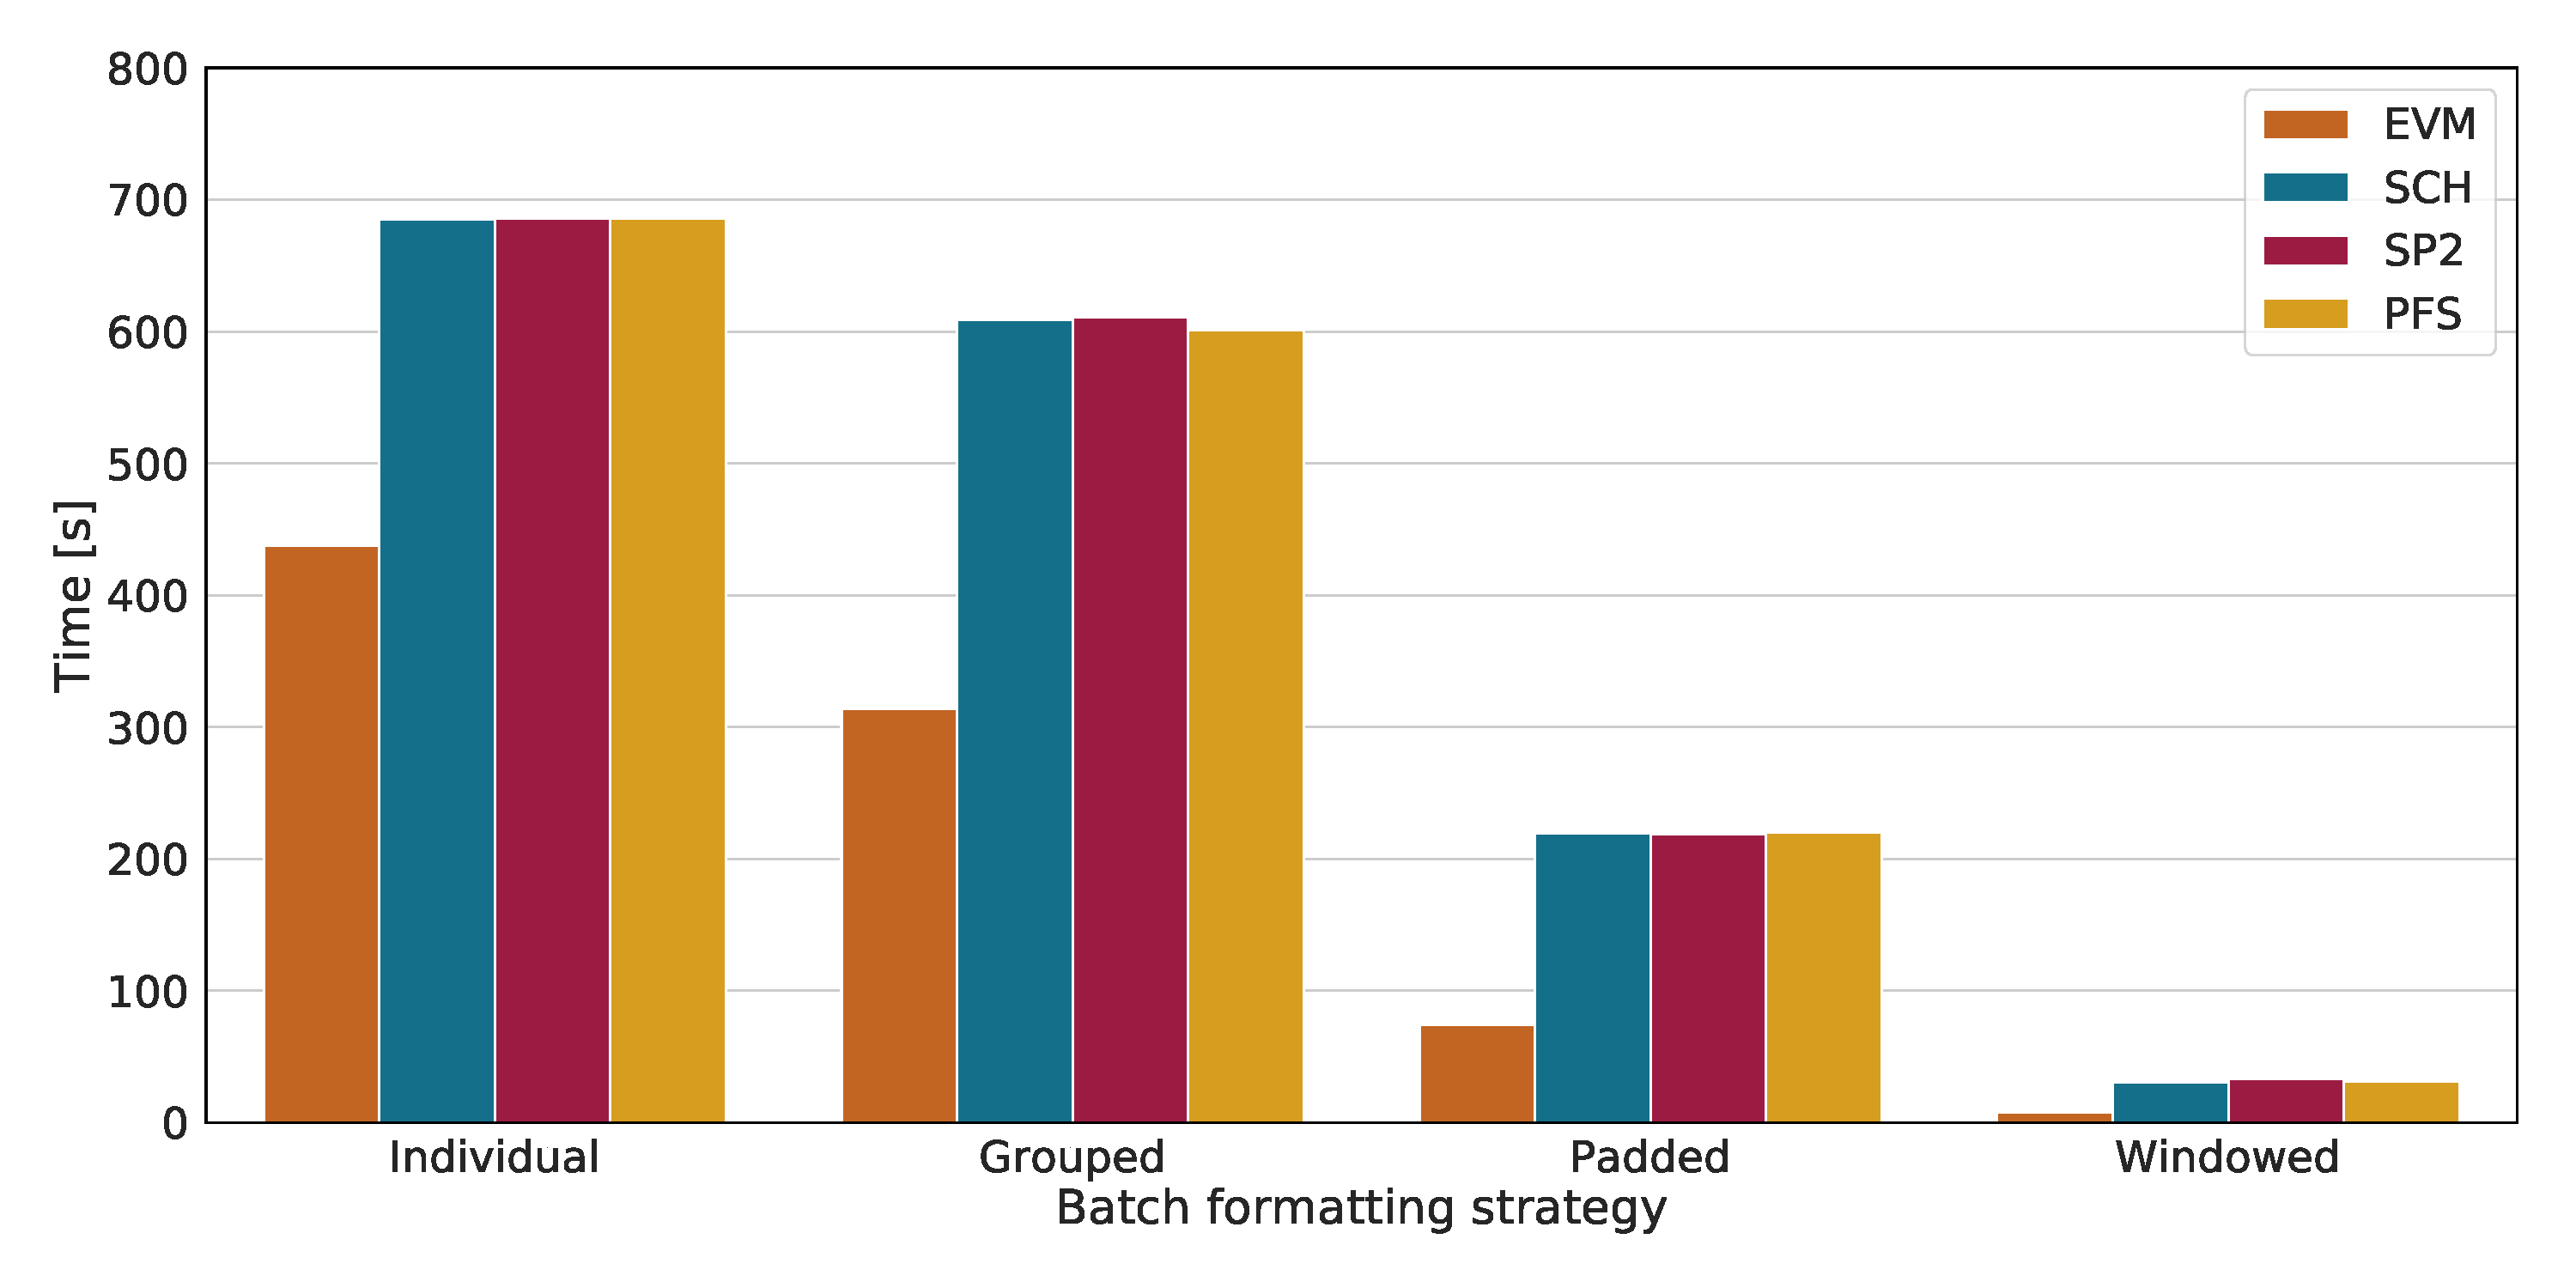
\includegraphics[width=\textwidth]{gfx/bpic2011/train_timings.pdf}
    \caption{Training times measured on BPIC11}
    \label{fig:BPIC11-training-timings}
\end{figure}
\begin{figure}
    \centering
    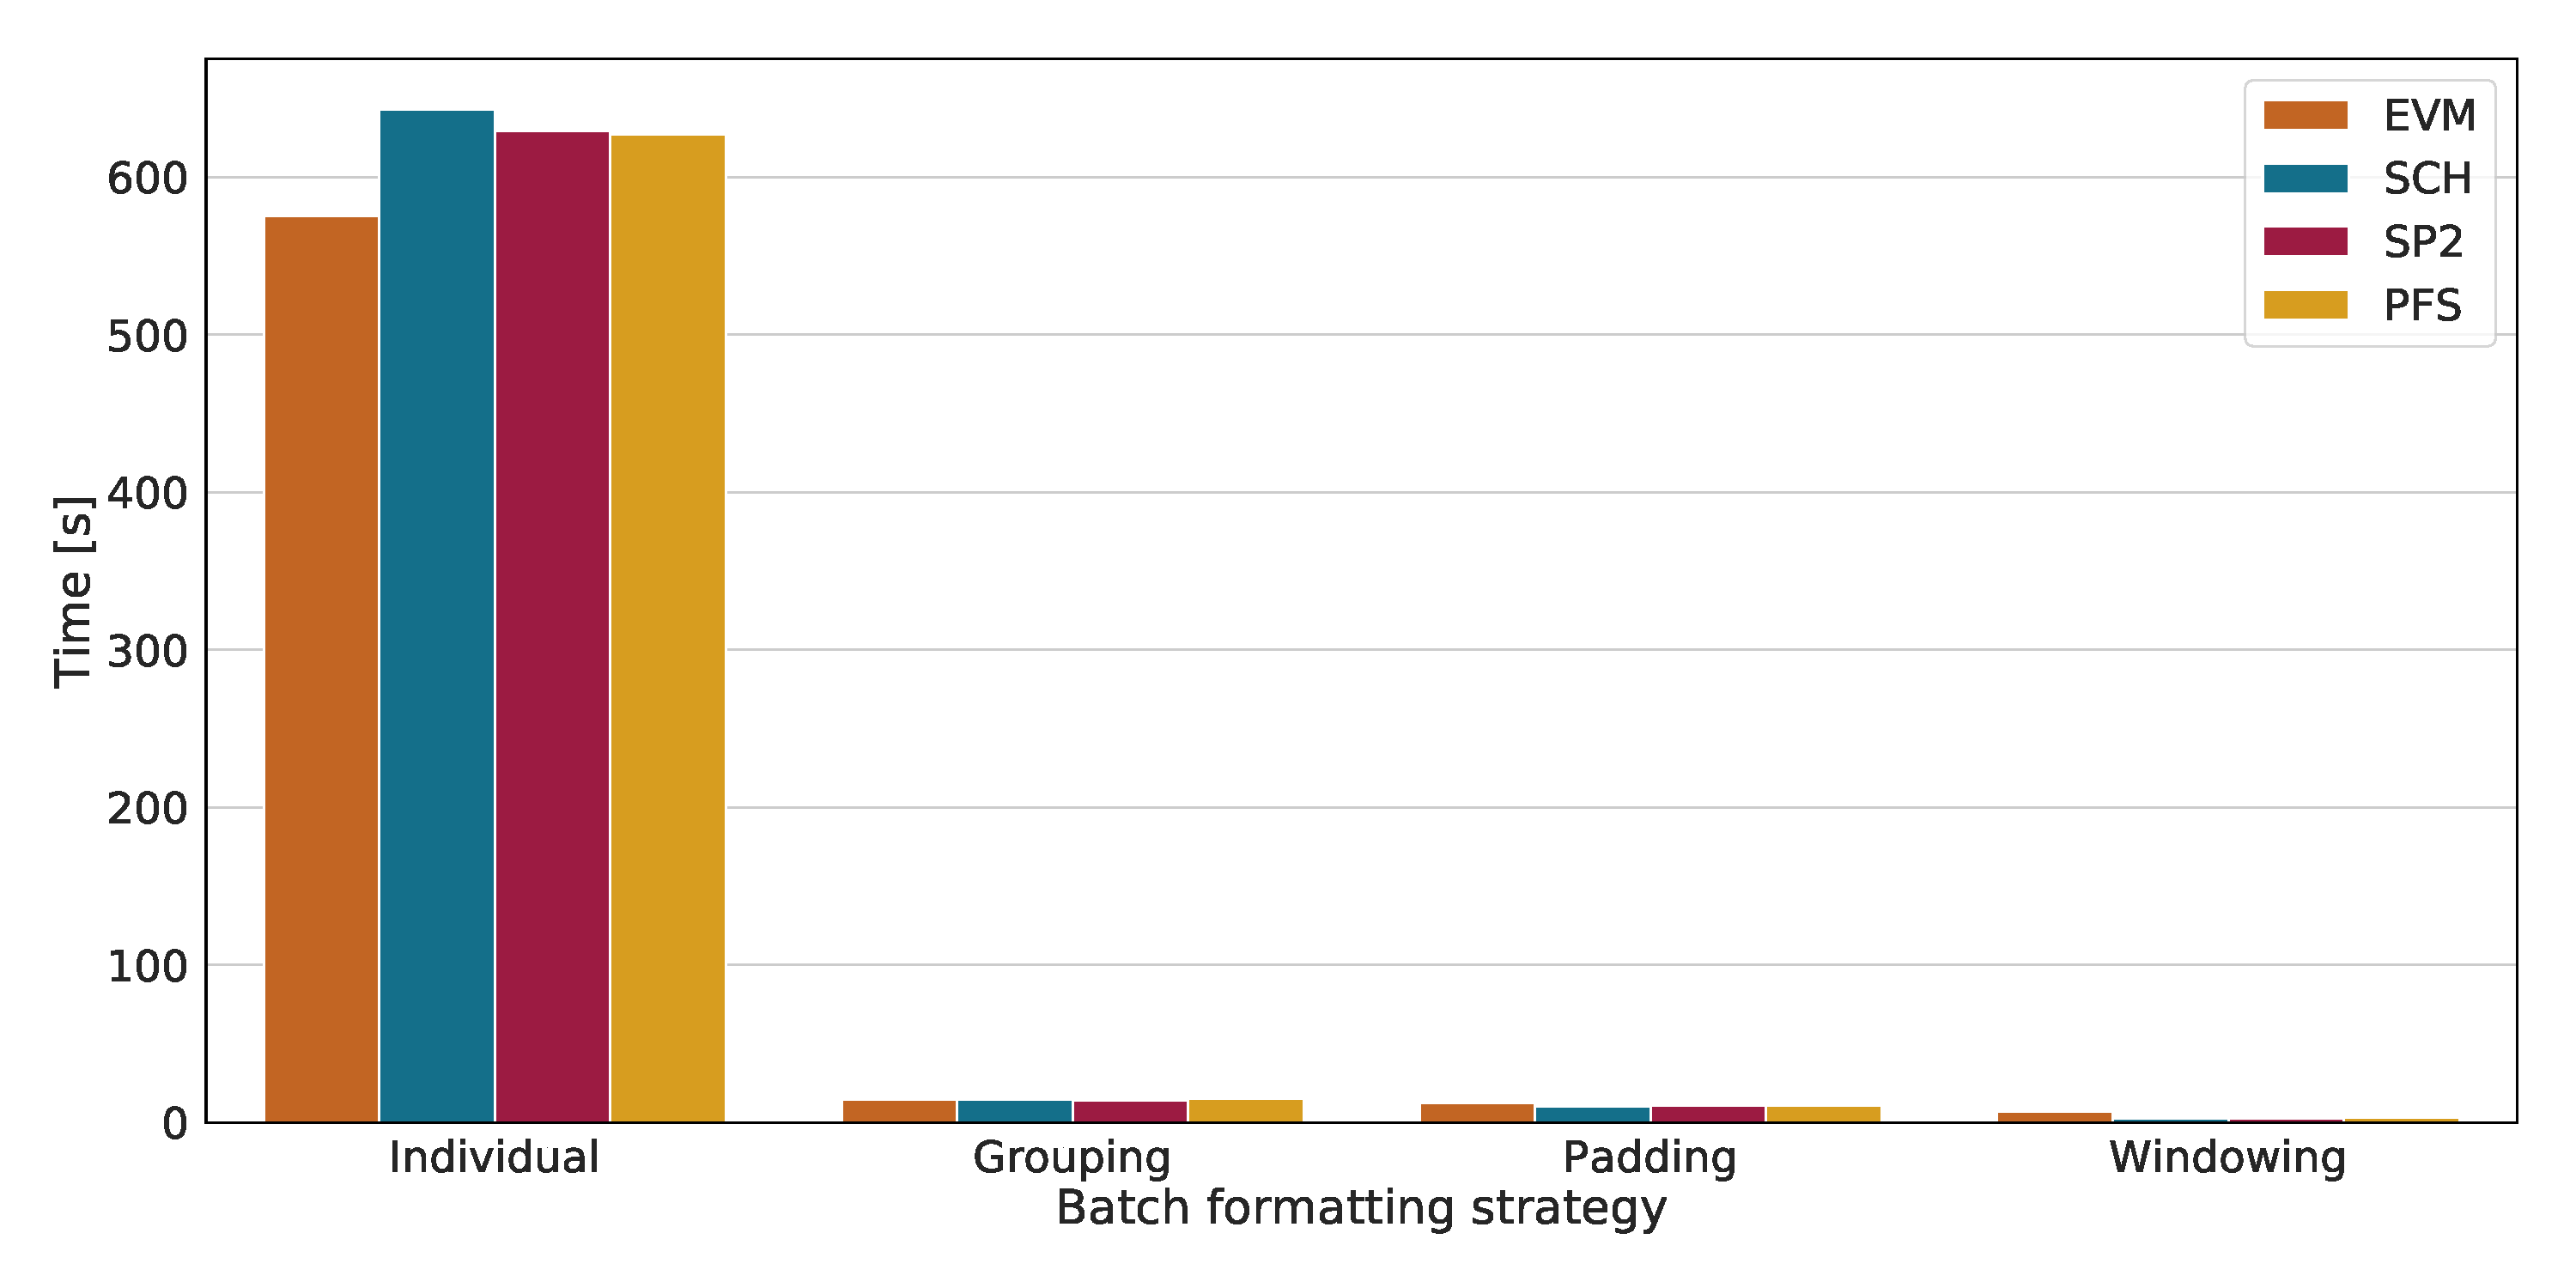
\includegraphics[width=\textwidth]{gfx/bpic2012/train_timings.pdf}
    \caption{Training times measured on BPIC12}
    \label{fig:BPIC12-training-timings}
\end{figure}
\begin{figure}
    \centering
    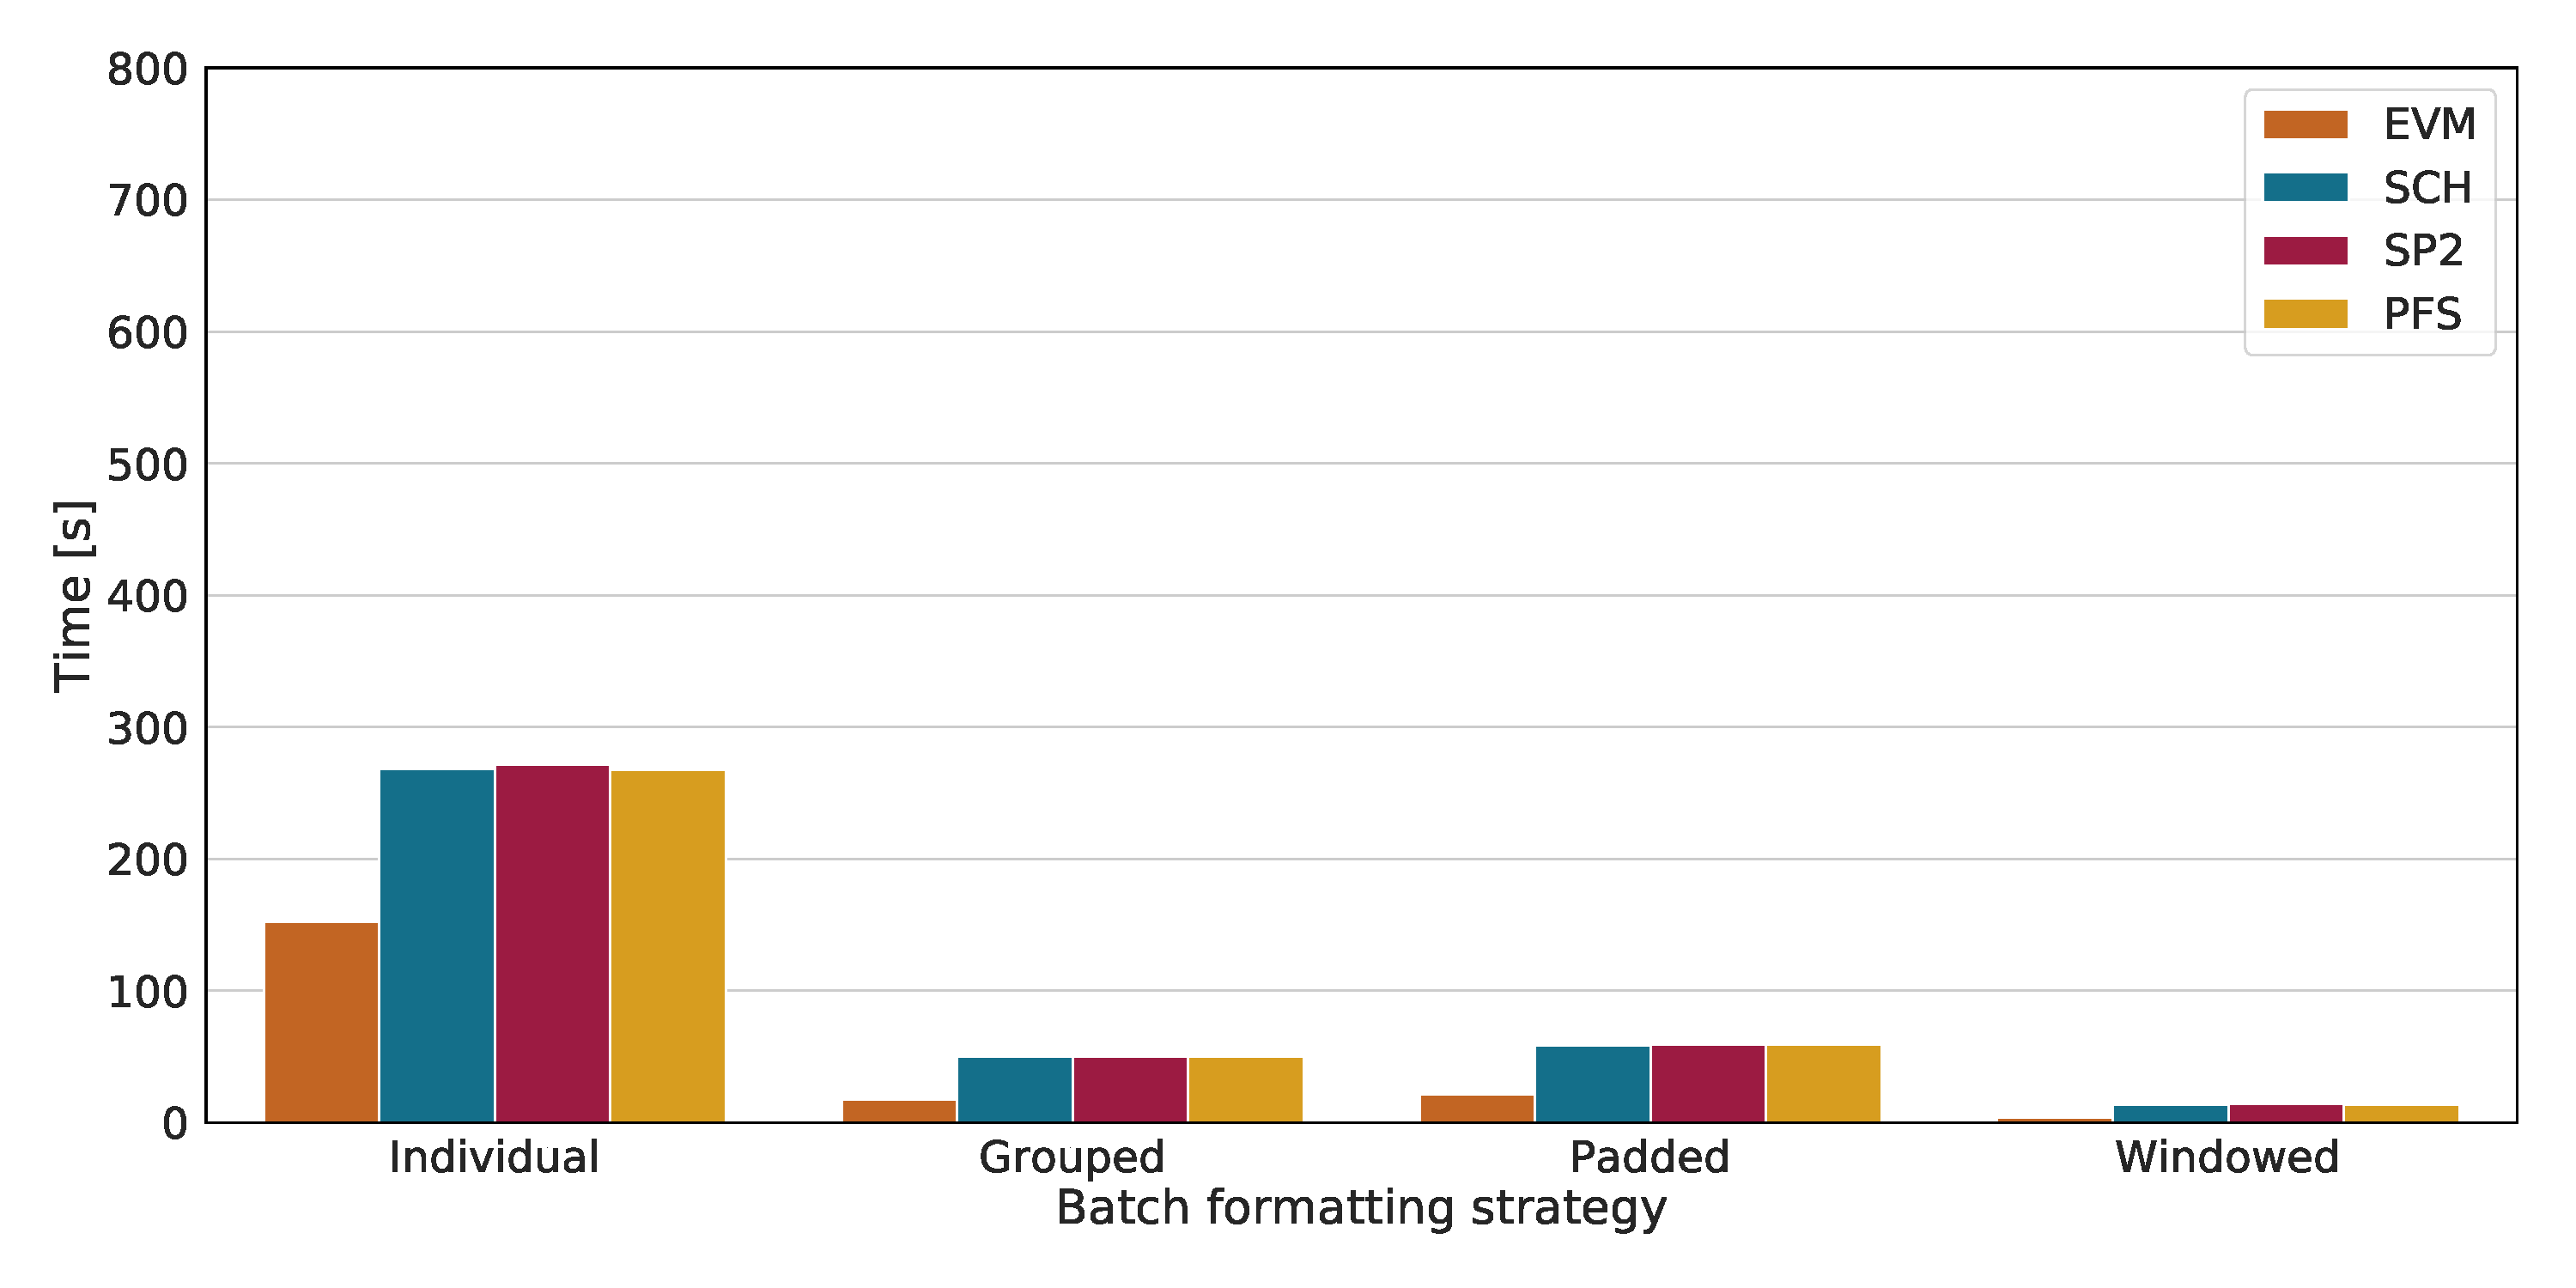
\includegraphics[width=\textwidth]{gfx/bpic2015_1/train_timings.pdf}
    \caption{Training times measured on BPIC15-1}
    \label{fig:BPIC15-1-training-timings}
\end{figure}
\begin{figure}
    \centering
    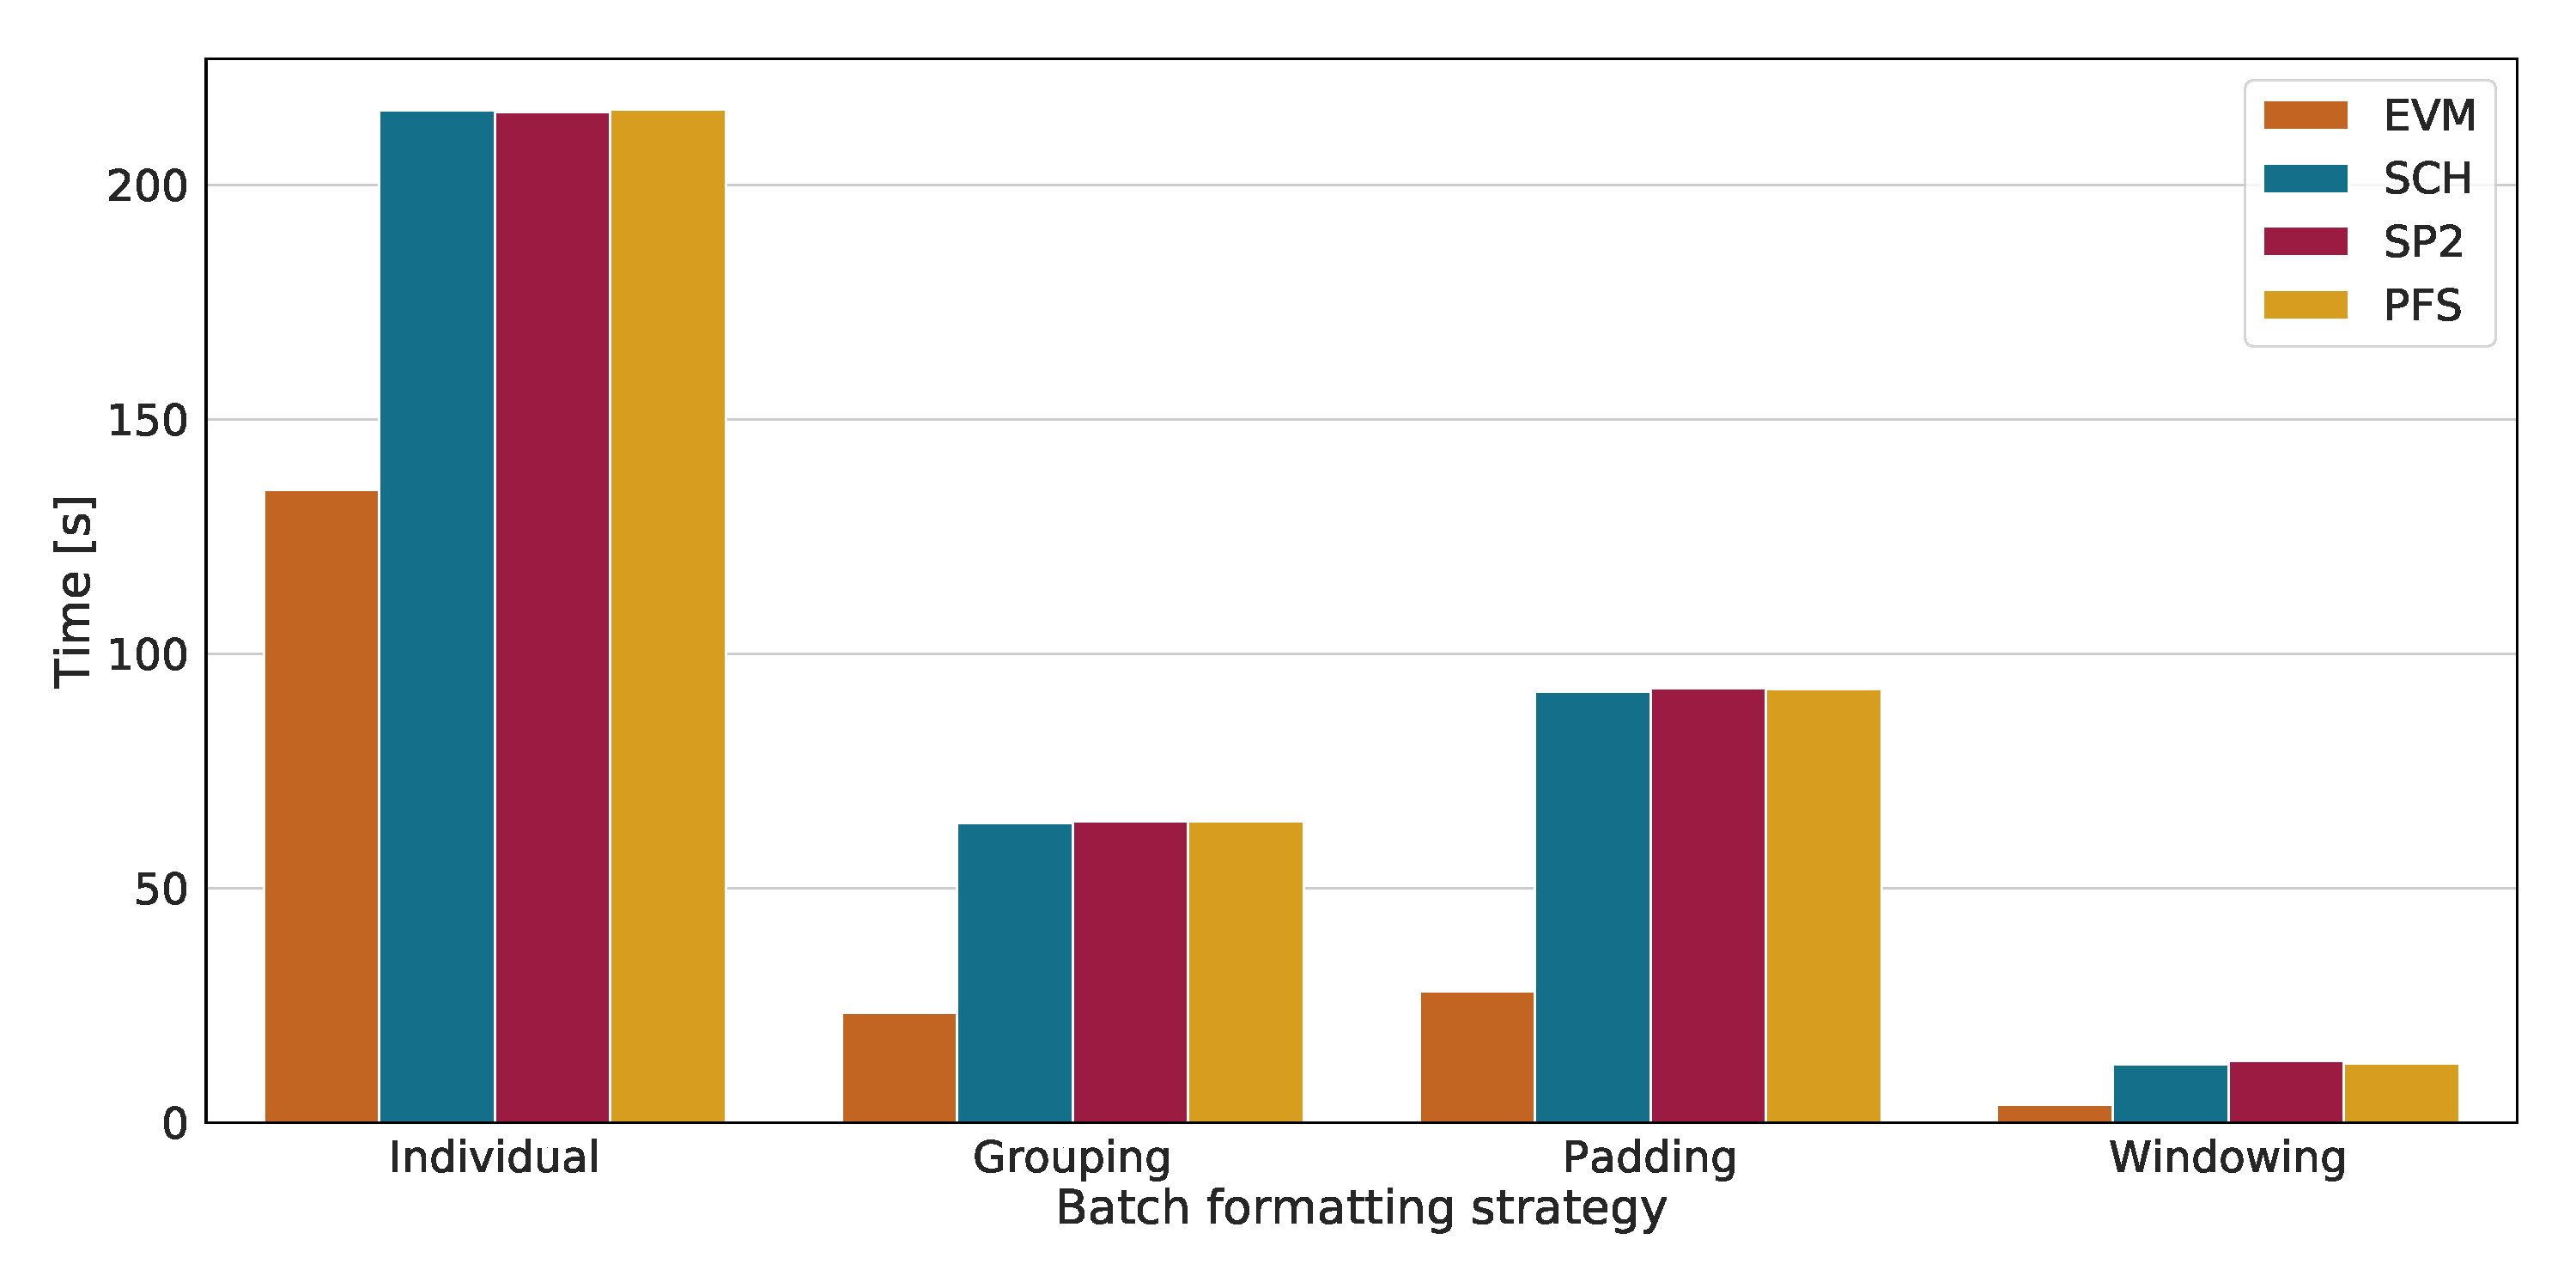
\includegraphics[width=\textwidth]{gfx/bpic2015_2/train_timings.pdf}
    \caption{Training times measured on BPIC15-2}
    \label{fig:BPIC15-2-training-timings}
\end{figure}
\begin{figure}
    \centering
    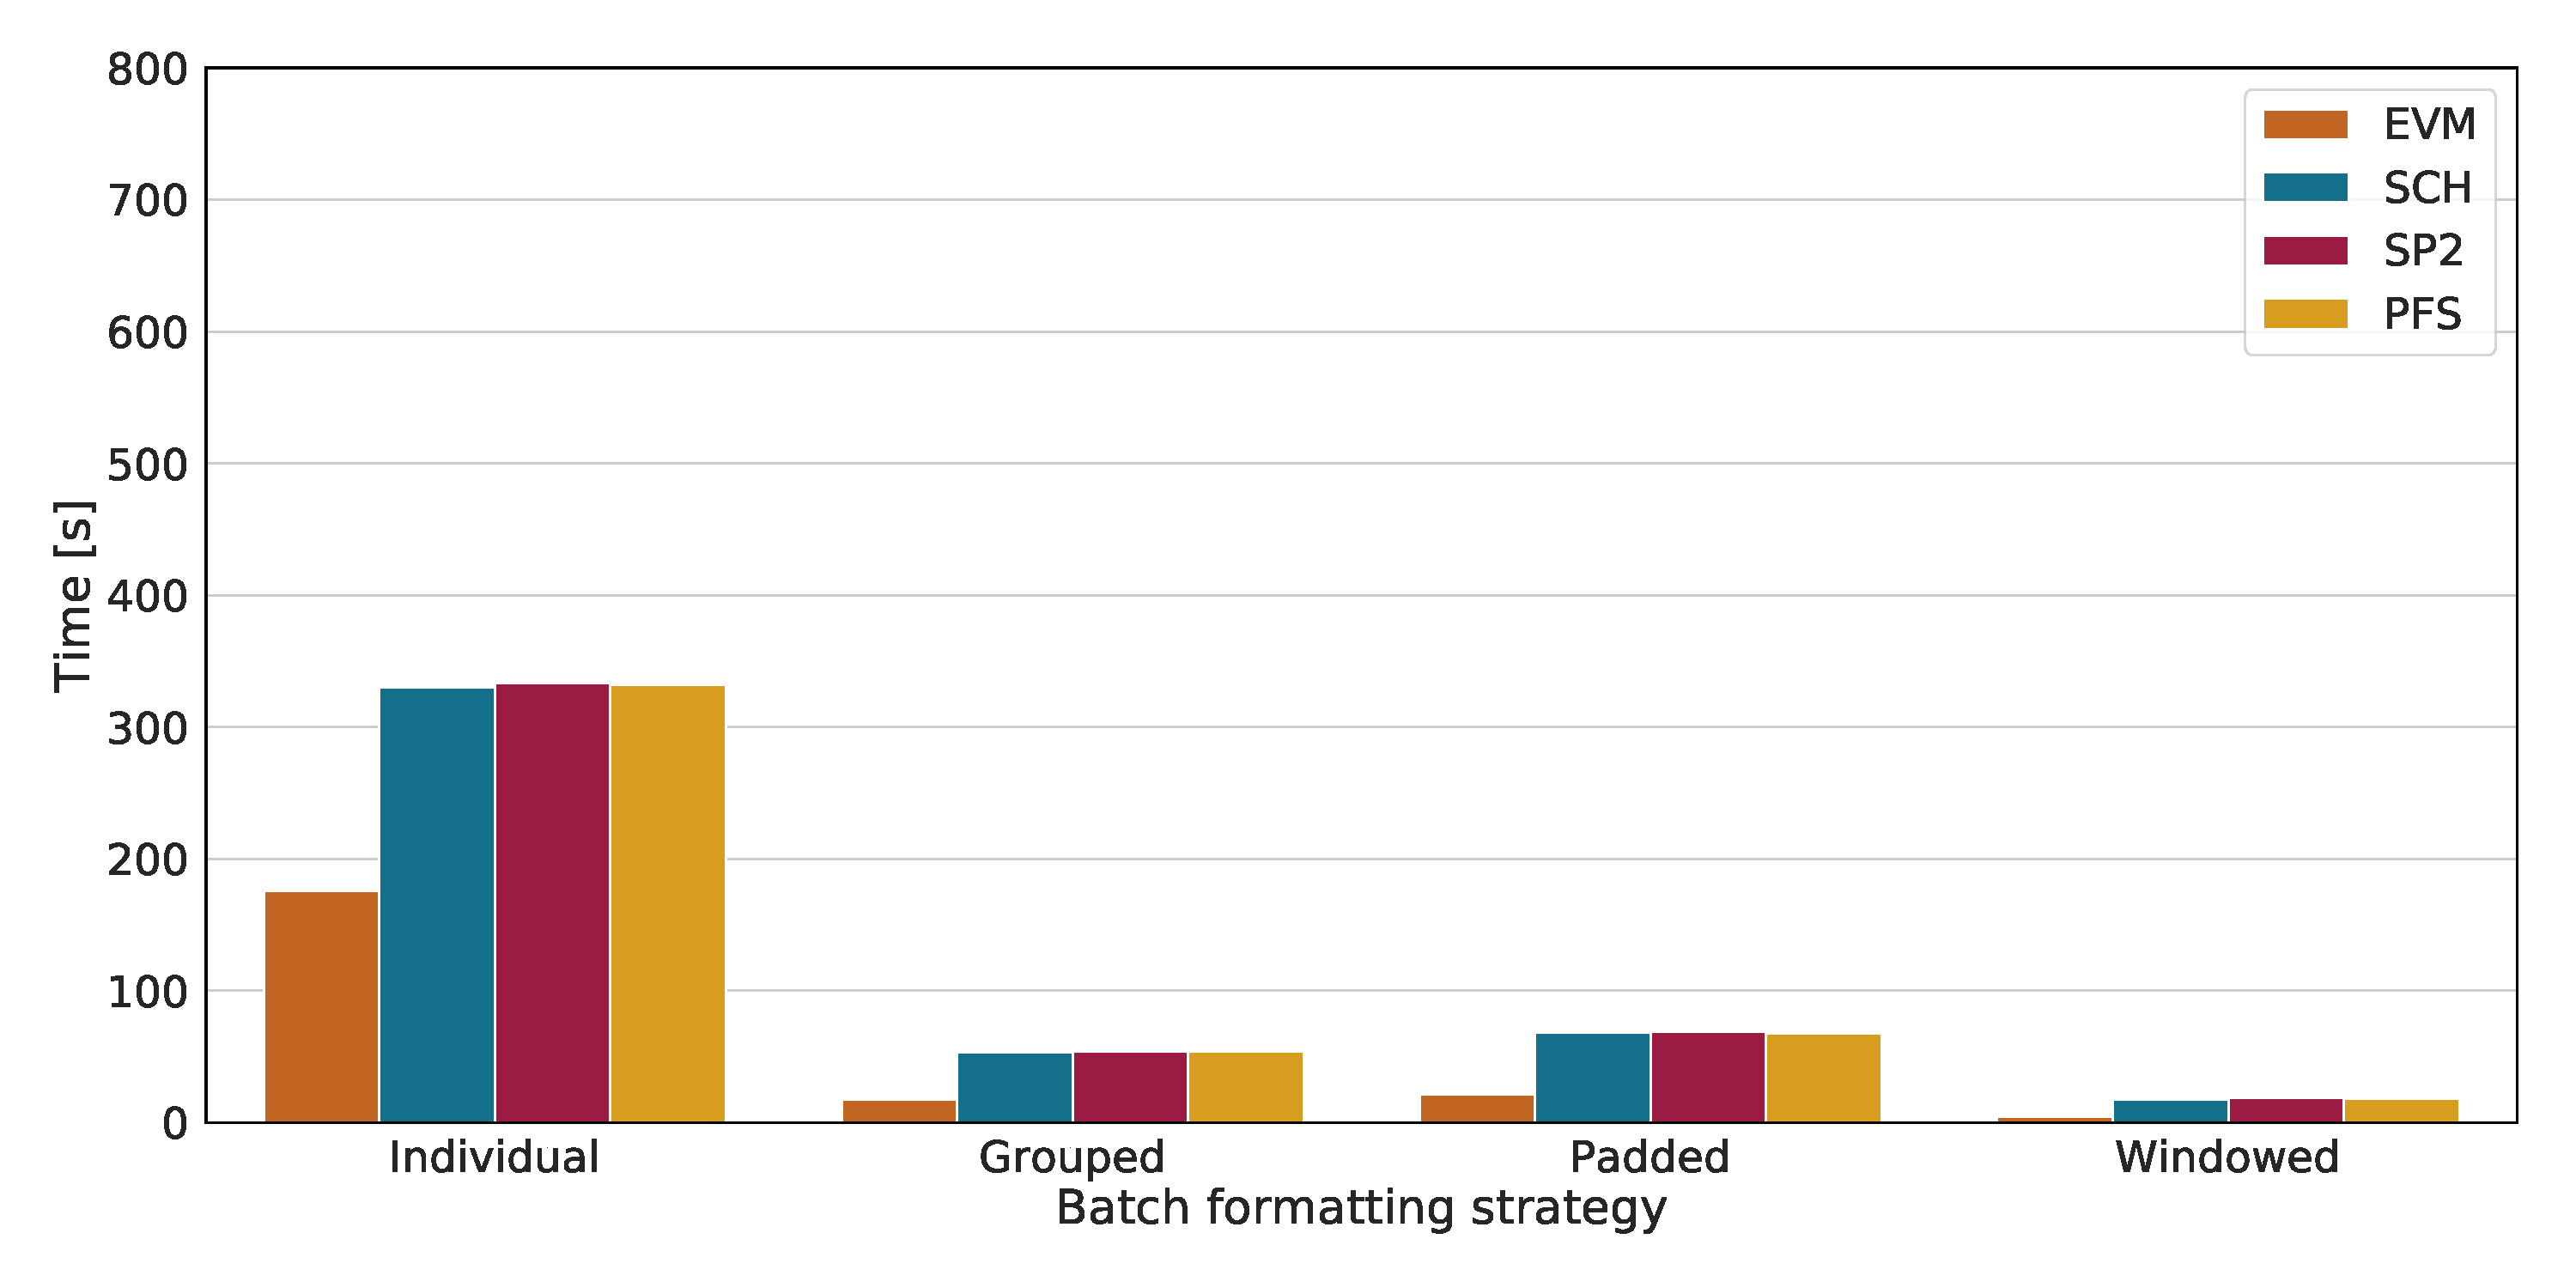
\includegraphics[width=\textwidth]{gfx/bpic2015_3/train_timings.pdf}
    \caption{Training times measured on BPIC15-3}
    \label{fig:BPIC15-3-training-timings}
\end{figure}
\begin{figure}
    \centering
    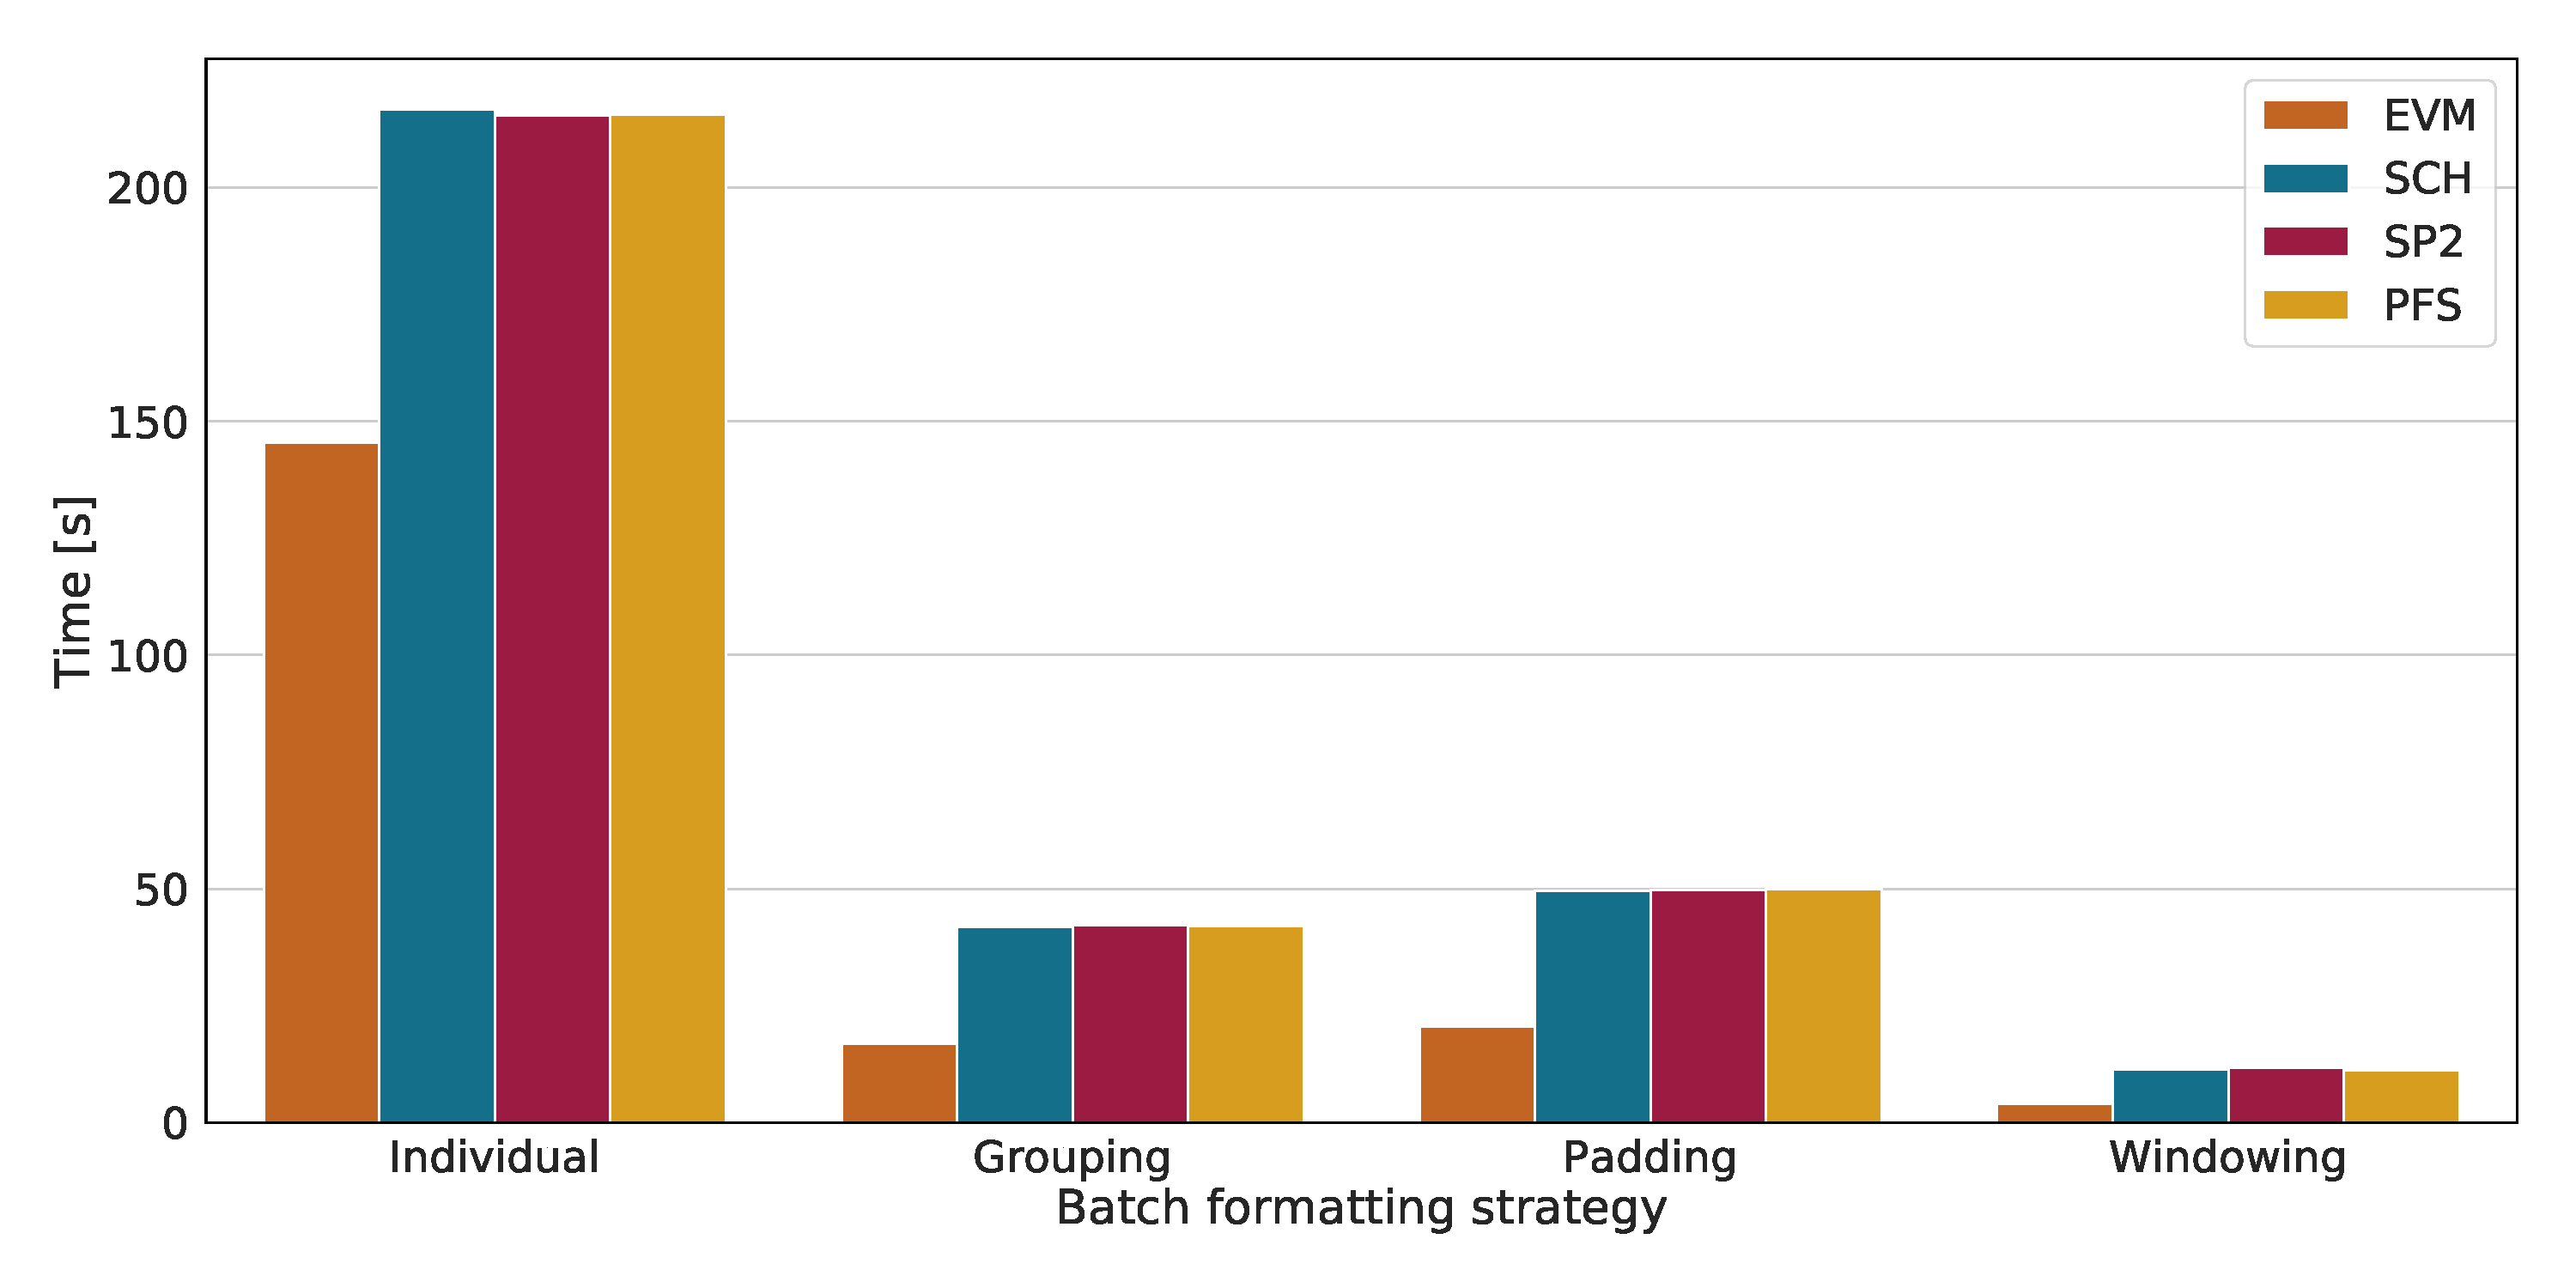
\includegraphics[width=\textwidth]{gfx/bpic2015_4/train_timings.pdf}
    \caption{Training times measured on BPIC15-4}
    \label{fig:BPIC15-4-training-timings}
\end{figure}
\begin{figure}
    \centering
    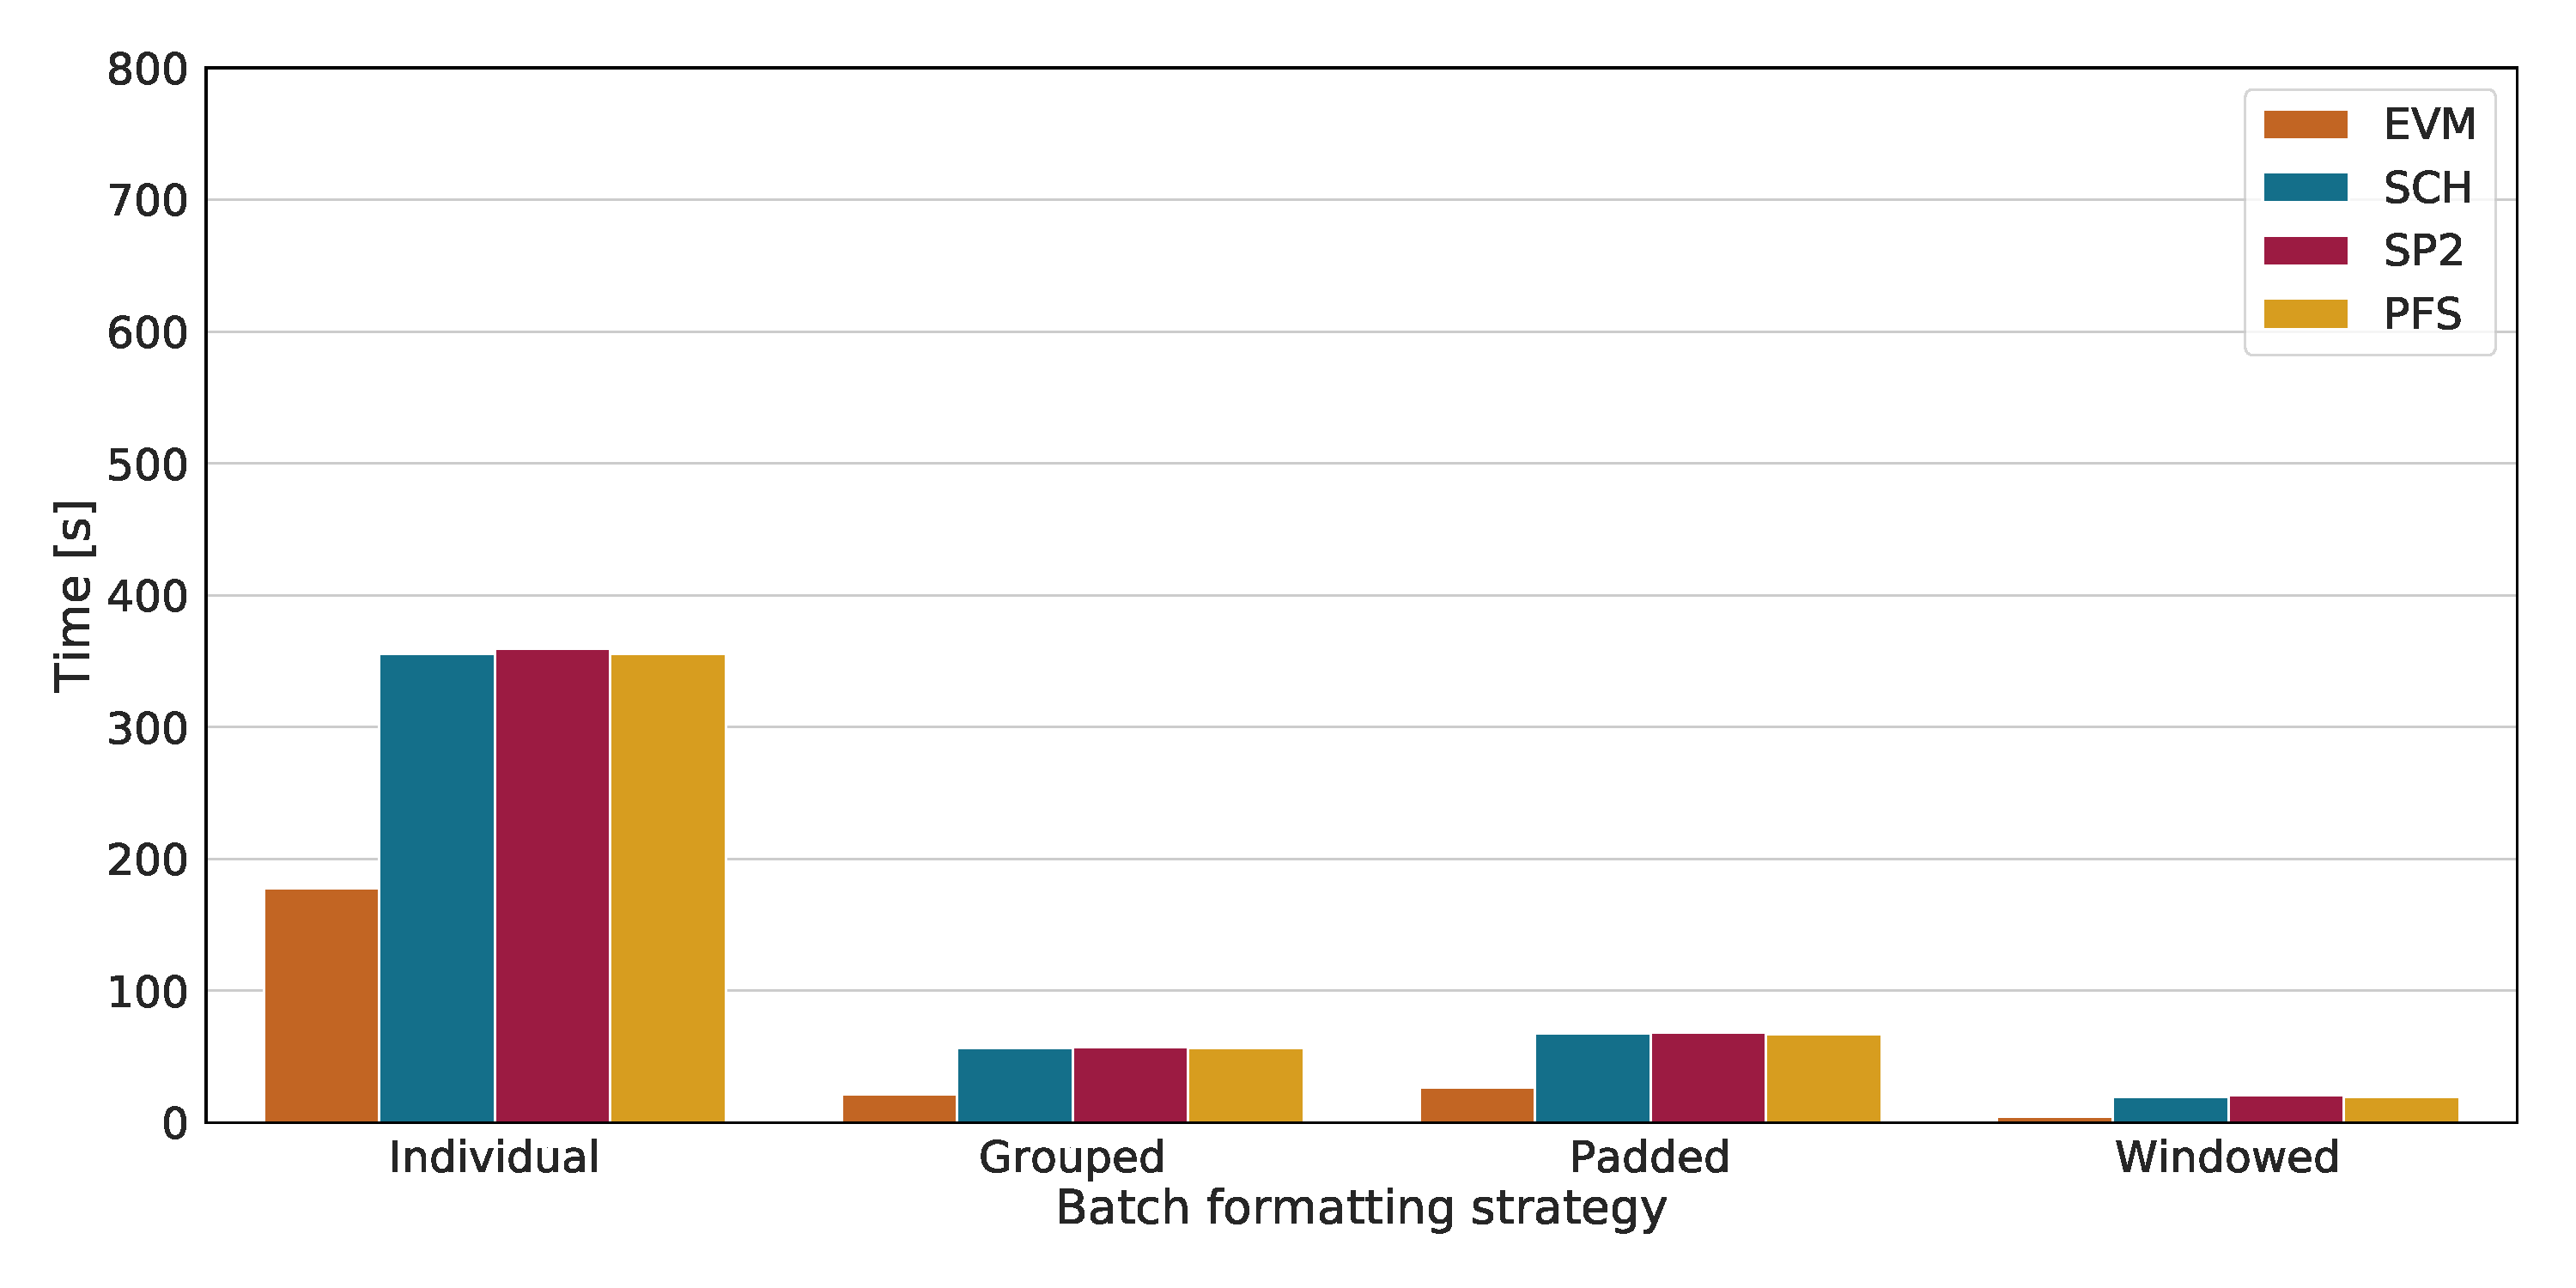
\includegraphics[width=\textwidth]{gfx/bpic2015_5/train_timings.pdf}
    \caption{Training times measured on BPIC15-5}
    \label{fig:BPIC15-5-training-timings}
\end{figure}
\FloatBarrier

\section{Stability}\label{sec:eval:stability}
As we stressed in the introduction, the stability of a prediction model along the progress of a case greatly impacts the level of trust that users put into the model~\cite{metzger2015}. \autoref{appendix:evaluation-measurements} contains the figures that illustrate the stability of each model per batching strategy, grouped by dataset. Each figure for a batching strategy and a dataset contains four curves, one for each model. The curves show the model accuracy along the progression of all traces inside the validation set in steps of $5\%$. The stability on the HelpDesk log was calculated in steps of $10\%$, as most cases in it are only 13 steps long. This subsection explains the results, again per batching strategy.\\

The individual batching strategy not only takes the most time, but it also leads to strong differences between the SCH, SP2, and PFS models. A good example is the difference between \autoref{fig:bpic15-3-individual-stability} and \autoref{fig:bpic15-3-grouped-stability}. In the latter figure, the SCH, SP2 and PFS curves are a lot closer to each other.

The grouping strategy increases the sample count per batch, and this seems to have a harmonizing effect on the results as evidenced by the corresponding figures of all datasets. This harmonizing effect is manifested in the reduction of the standard deviation of the best accuracies of the SCH, SP2 and PFS models in \autoref{fig:grouping-accuracy-harmonization}.

\begin{figure}
    \centering
    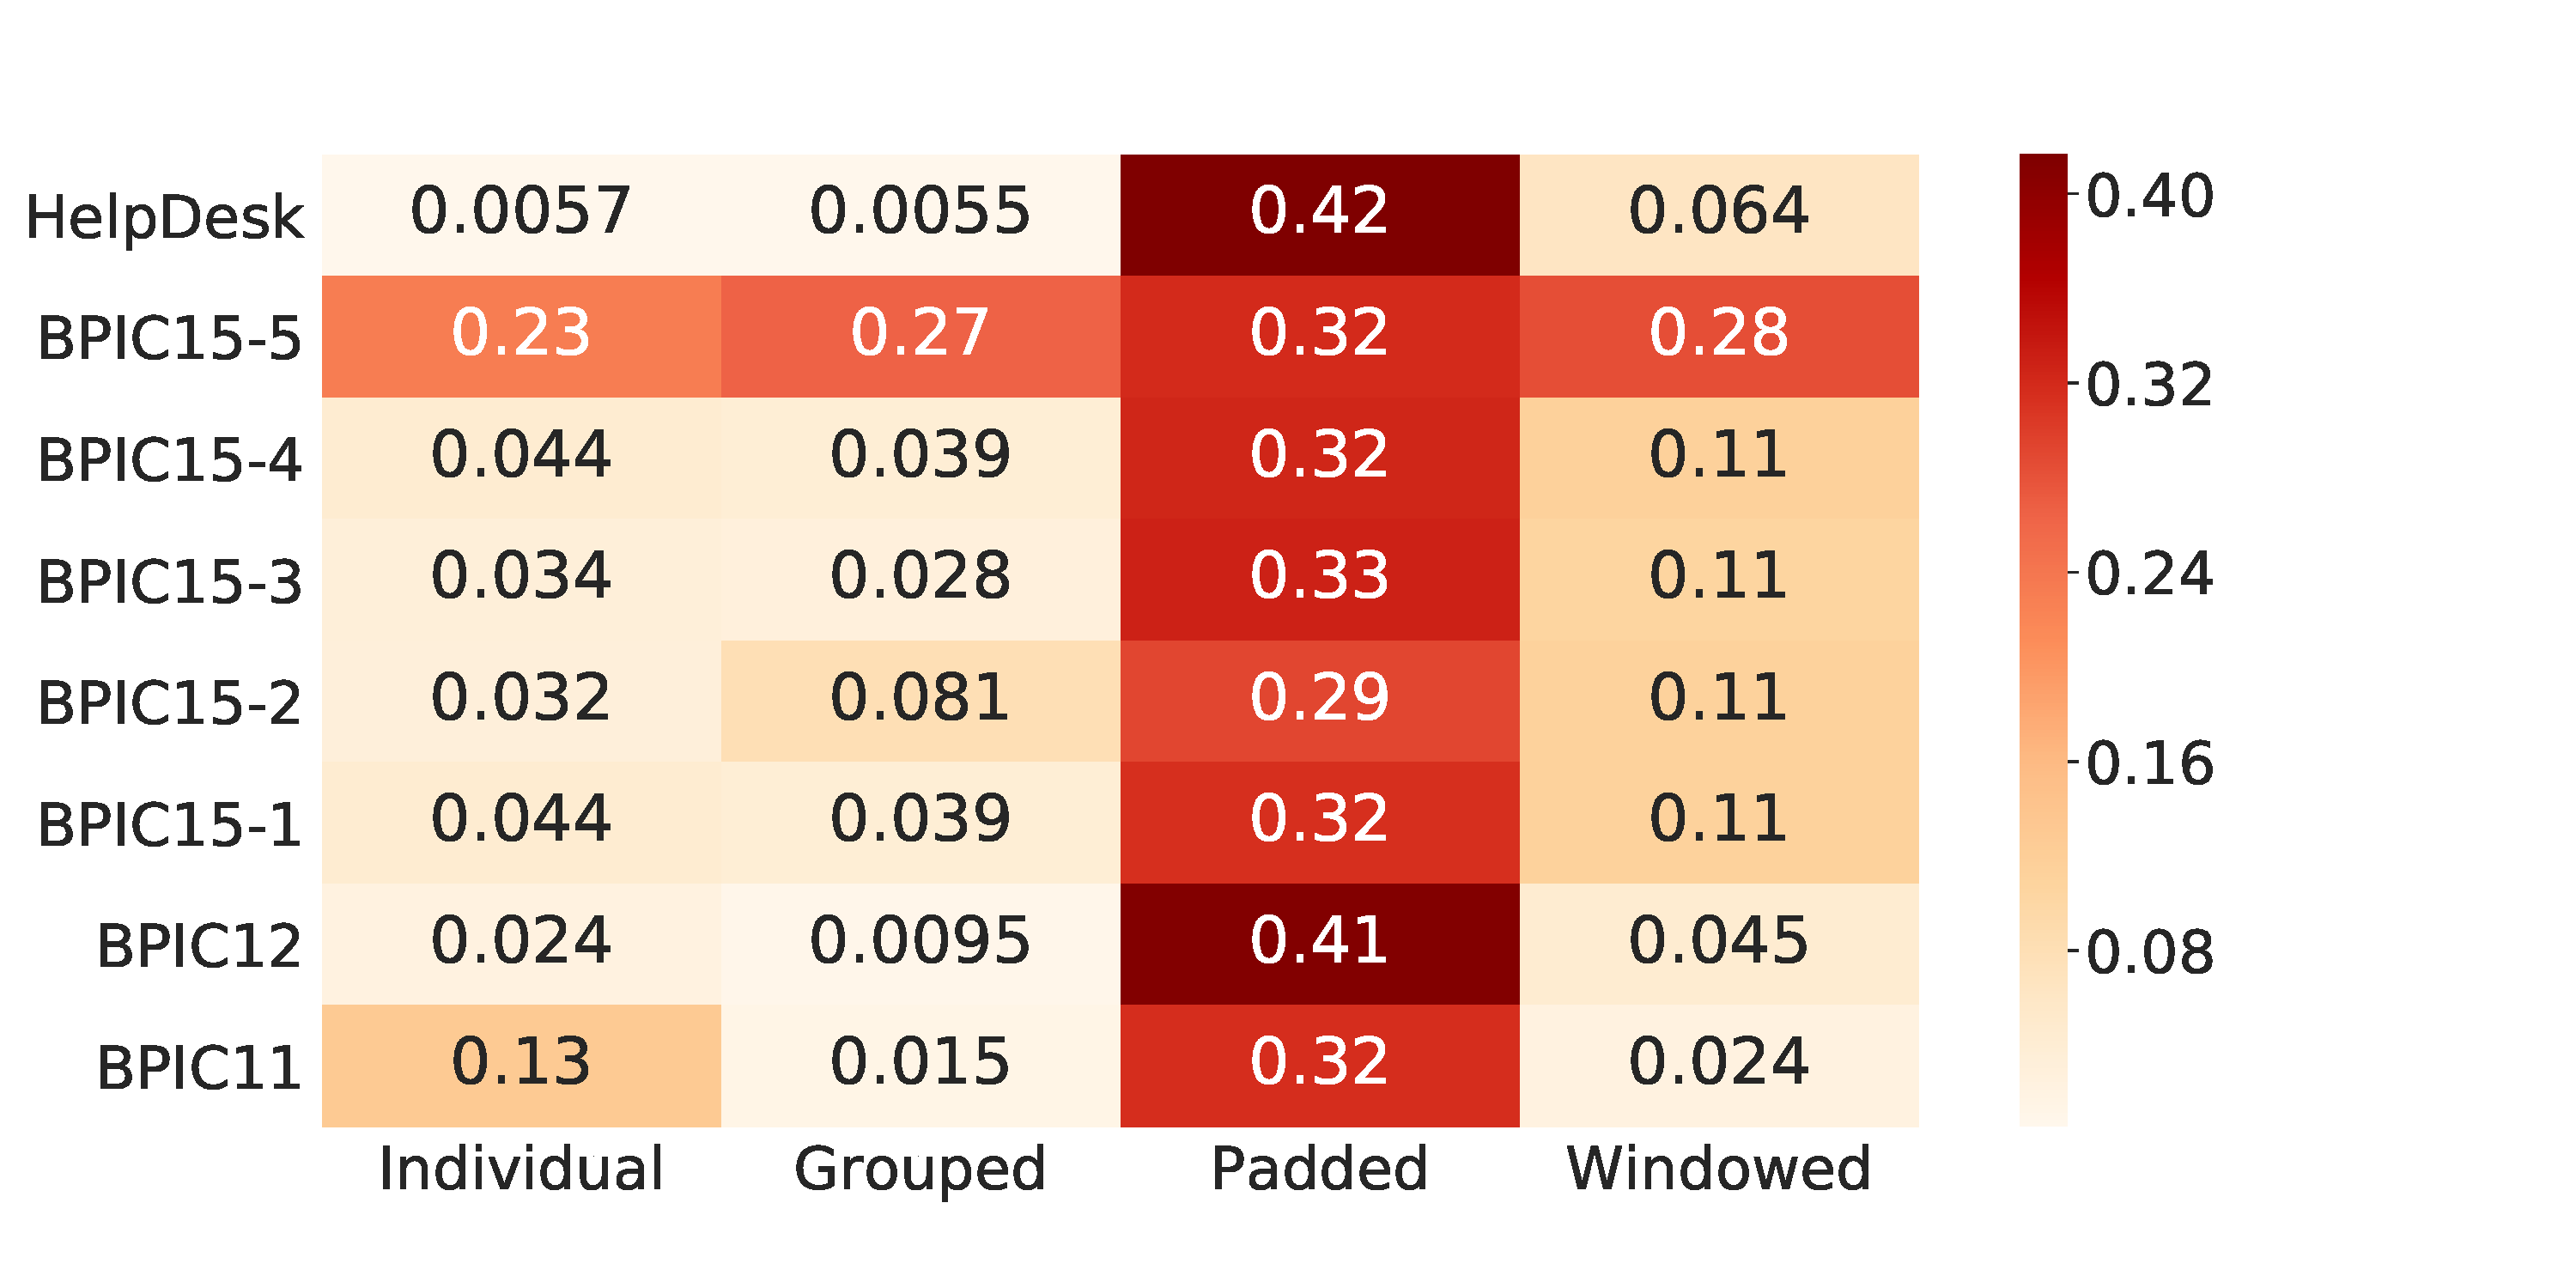
\includegraphics[width=\textwidth]{gfx/grouping-accuracy-harmonization.pdf}
    \caption[Batching strategy harmonizes top accuracies]{The grouping strategy often reduces the standard deviation between the highest accuracies of SCH, SP2 and PFS models}
    \label{fig:grouping-accuracy-harmonization}
\end{figure}

The padded strategy yields results that are very similar to the grouped strategy - except on BPIC11 and HelpDesk. In the former case, the training data had to be trimmed because the padded traces had required too much memory. In the latter case, the batch size seems to have had a profound effect on accuracy.

Klinkmüller et al. state that the windowing strategy leads to unstable results~\cite{klinkmuller2018reliablemonitoring}. While this statement seems to be especially true for the longer processes in BPIC11 and BPIC15, the windowing strategy seems to have less of an impact with shorter processes as evidenced with BPIC12. There, all models show a dip towards the end of the trace.\\

Generally, models were expected to become more accurate as the trace neared its end. However, this did not turn out to be the case. Instead, the accuracy was high when variability in the respective stage of the process was low. For example, processes in BPIC11 always begin similarly, as patients need to be onboarded~\cite{bose2011analysis}. The connection of accuracy and variability could be a cause for the high accuracies at the beginning of the BPIC11 stability curves. The processes in BPIC12 always end either on approval or dismissal of the application, making the models very accurate in this stage~\cite{adriansyah2012mining}.

\section{Discussion}\label{sec:eval:discussion}
After presenting and explaining our findings, we summarize our learnings in this section and compare our findings to the papers mentioned in \autoref{sec:method:dataset-choice}.\\

First, we can to confirm Klinkmüller et al.~\cite{klinkmuller2018reliablemonitoring} and their suspicion that windowed batching does not work well for sequence prediction. While it may be a performant strategy to use for time-series prediction, it does not work very well for predicting the future of a single case.

Second, we find that the grouping strategy frequently delivers the best results in terms of speed and accuracy. We realized that it should be iterated upon to include a threshold which limits batches to a maximum size and splits the larger batches accordingly. As evidenced by the charts, the grouping strategy seems to perform better with a medium to highly complex processes from BPIC11 and BPIC15, while padding works better with the more straightforward process from BPIC12. In combination with the SP2 model, the grouping strategy contributed to most of the highest accuracies.

Third, we realize that Embeddings might not be useful on the currently available datasets as these might have not enough samples. The lacking performance of the EVM model and its barely converging loss indicate that this might be the case. All accuracy/loss curves from training are enclosed in \autoref{appendix:loss-curves}, and show that especially for the EVM model, the loss optimization does not work correctly.\\

We end the evaluation with a comparison of our best results with the initially mentioned publications based on BPIC12. While Evermann et al.~\cite{evermann2016} were able to obtain an accuracy of $0.768$, they did not focus on specific cases. Furthermore, Evermann et al. did not use Keras on top of Tensorflow but Tensorflow directly, which enabled him to make use of low-level functions directly. To the best of our knowledge, our implementation sufficiently approximates theirs, but this can be a reason for the low accuracy. Another very probable reason is their feature engineering~\cite{evermann2016}.

On BPIC12 and the HelpDesk log, Böhmer et al.~\cite{boehmer2018probability} attain an accuracy of $0.77$ with their statistical approach. While they argue that machine learning methods may perform better, they place great value on comprehensible reasoning information from the model.

Tax et al.~\cite{tax2017} reach a maximum accuracy of $0.76$ in their paper on BPIC12 and $0.71$ on the HelpDesk log.

Using the individual batching strategy, all SCH, SP2, and PFS score above $0.80$ on both datasets.
This surpasses all three aformentioned results.
The SCH model edges to the best accuracy of $0.853$, with the SP2 model close at $0.851$ on BPIC12.
On the HelpDesk dataset, the PFS and SCH models reach $0.862$ and $0.854$.
The fact that our accuracy surpasses that of Böhmer et al. supports their thesis of lower comprehensibility at higher accuracy.\\

In this evaluation we discussed the performances of the models on the individual datasets.
We determined that the grouping strategy delivers good results, but can still be optimized.
Furthermore, we noted that the complexity of the traces in the log has a large impact on stability.
Depending on the amount of variability in different stages of the process, model accuracy varies dramatically.
We could confirm that our models outperform recently published approaches, and describe how it can be improved in the next chapter.
We then conclude the thesis with a summary of the results.
